\documentclass[a4paper,12pt]{article}
\usepackage[utf8]{inputenc}
\usepackage[a4paper,
            bindingoffset=0.2in,
            left=1in,
            right=1in,
            top=1in,
            bottom=1in,
            footskip=.25in]{geometry}


%###############################################################################

%\input{~/layout/global_layout}


%###############################################################################

% packages begin

\usepackage[
  backend=biber,
  sortcites=true,
  style=alphabetic,
  eprint=true,
  backref=true
]{biblatex}
\addbibresource{bibliography.bib}

\usepackage{euscript}[mathcal]
% e.g. \mathcal{A} for fancy letters in mathmode
\usepackage{amsmath,amssymb,amstext,amsthm}

\usepackage{mdframed}
\newmdtheoremenv[nobreak=true]{problem}{Problem}[subsection]
\newmdtheoremenv[nobreak=true]{claim}{Claim}[subsection]
\newtheorem{definition}{Definition}[subsection]
\newtheorem{lemma}{Lemma}[claim]
\newtheorem{plemma}{Lemma}[problem]

\usepackage{mathtools}
\DeclarePairedDelimiter\ceil{\lceil}{\rceil}
\DeclarePairedDelimiter\floor{\lfloor}{\rfloor}

\usepackage{enumerate}
\usepackage[pdftex]{graphicx}
\usepackage{subcaption}
% 'draft' für schnelleres rendern mitübergeben -> [pdftex, draft]
% dadruch wird nicht das bild mitgerendered, sondern nur ein kasten mit bildname -> schont ressourcen

\usepackage{hyperref}

\usepackage{tikz}
\usetikzlibrary{arrows,automata,matrix,positioning,shapes}

% for adding non-formatted text to include source-code
\usepackage{listings}
\lstset{language=Python,basicstyle=\footnotesize}
% z.B.:
% \lstinputlisting{source_filename.py}
% \lstinputlisting[lanugage=Python, firstline=37, lastline=45]{source_filename.py}
%
% oder
%
% \begin{lstlisting}[frame=single]
% CODE HERE
%\end{lstlisting}
\usepackage{algorithm}
\usepackage{algpseudocode}

\usepackage{wasysym}

\usepackage{titling}
\usepackage{titlesec}
\usepackage[nocheck]{fancyhdr}
\usepackage{lastpage}

\usepackage{kantlipsum}
\usepackage[colorinlistoftodos,prependcaption,textsize=tiny]{todonotes}

% packages end
%###############################################################################

\pretitle{% add some rules
  \begin{center}
    \LARGE\bfseries
} %, make the fonts bigger, make the title (only) bold
\posttitle{%
  \end{center}%
  %\vskip .75em plus .25em minus .25em% increase the vertical spacing a bit, make this particular glue stretchier
}
\predate{%
  \begin{center}
    \normalsize
}
\postdate{%
  \end{center}%
}

\titleformat*{\section}{\Large\bfseries}
\titleformat*{\subsection}{\large\bfseries}
\titleformat*{\subsubsection}{\normalsize\bfseries}

\titleformat*{\paragraph}{\Large\bfseries}
\titleformat*{\subparagraph}{\large\bfseries}

%###############################################################################
% TODO define Headers and Fotter

\pagestyle{fancy}
\fancyhf{}
% l=left, c=center, r=right; e=even_pagenumber, o=odd_pagenumber; h=header, f=footer
% example: [lh] -> left header, [lof,ref] -> fotter left when odd, right when even
%\fancyhf[lh]{}
%\fancyhf[ch]{}
%\fancyhf[rh]{}
%\fancyhf[lf]{}
\fancyhf[cf]{\footnotesize Page \thepage\ of \pageref*{LastPage}}
%\fancyhf[rf]{}
\renewcommand{\headrule}{} % removes horizontal header line

% Fotter options for first page

\fancypagestyle{firstpagestyle}{
  \renewcommand{\thedate}{\textmd{}} % removes horizontal header line
  \fancyhf{}
  \fancyhf[lh]{\ttfamily M.Sc. Computer Science\\KTH Royal Institute of Technology}
  \fancyhf[rh]{\ttfamily Period 3\\\today}
  \fancyfoot[C]{\footnotesize Page \thepage\ of \pageref*{LastPage}}
  \renewcommand{\headrule}{} % removes horizontal header line
}
%###############################################################################
% Todo: define Title

\title{
  \normalsize{DD2358 VT25 Introduction to}\\
  \normalsize{High Performance Computing}\\
  \large{Assignment 4 -- Optimization with Parallelization}\\
}
\author{
  \small Rishi Vijayvargiya\\[-0.75ex]
%  \footnotesize\texttt{MN: }\\[-1ex]
  \scriptsize\texttt{rishiv@kth.se}
  \and
  \small Lennart Herud\\[-0.75ex]
%  \footnotesize\texttt{MN: }\\[-1ex]
  \scriptsize\texttt{herud@kth.se}
  \and
  \small Paul Mayer\\[-0.75ex]
%  \footnotesize\texttt{MN: }\\[-1ex]
  \scriptsize\texttt{pmayer@kth.se}
  \and
  \small Adrian Sušec\\[-0.75ex]
%  \footnotesize\texttt{MN: }\\[-1ex]
  \scriptsize\texttt{susec@kth.se}
}
\date{}

%###############################################################################
% define Commands

\newcommand{\N}{\mathbb{N}}
\newcommand{\R}{\mathbb{R}}
\newcommand{\Z}{\mathbb{Z}}
\newcommand{\I}{\mathbb{I}}

\newcommand{\E}{\mathbb{E}}
\newcommand{\Prob}{\mathbb{P}}

\renewcommand{\epsilon}{\varepsilon}

% Todo: Set Counter to Excercise Sheet Number
% \setcounter{section}{4}
% \setcounter{subsection}{0}

%###############################################################################
%###############################################################################

\begin{document}
\maketitle
\thispagestyle{firstpagestyle}

\tableofcontents
\vspace{1em}

% content begin
%

%\setcounter{subsection}{1}
\section*{Code Repository}
The code for this assignment can be found in the following github repository: \url{https://github.com/paulmyr/DD2358-HPC25/tree/master/04_parallel}.

\section{Wildfire Spread in Parallel}
The code and associated files for Exercise 1 can be found under the \verb|exercisd1/| directory of the repository, here: \url{https://github.com/paulmyr/DD2358-HPC25/tree/master/04_parallel/exercise1}. The original, serial implementation provided to us is present in the \verb|wildfiremontecarloserial.py| file. This code has been modified and has additional function to run multiple simulations, along with code to save the grid output at certain intervals for the VTK visualization. All the results and runtimes that follow were obtained an a 2021 M1 MacBook Pro (16 inch), which has 10 cores. More information on its specifications are \href{https://support.apple.com/en-us/111901}{here}.

Since the essence of this task required us to run multiple visualizations, we refrain from outputting the visualization of the grid for each simulation at certain intervals. Instead, at the end of the simulation (for all implementations), we plot a line graph showing dotted lines with the number of burned trees for all simulations, along with a darker line showing the average number of trees burned per day using the data from all simulations. To make sure that the results are reproducible, we use seeds from 0 to $n-1$ for $n$ simulations for all implementations. 

With this method, we get the following line-plot for the \textbf{serial implementation}, where we ran 5 simulations


\begin{figure}[H]
  \centering
  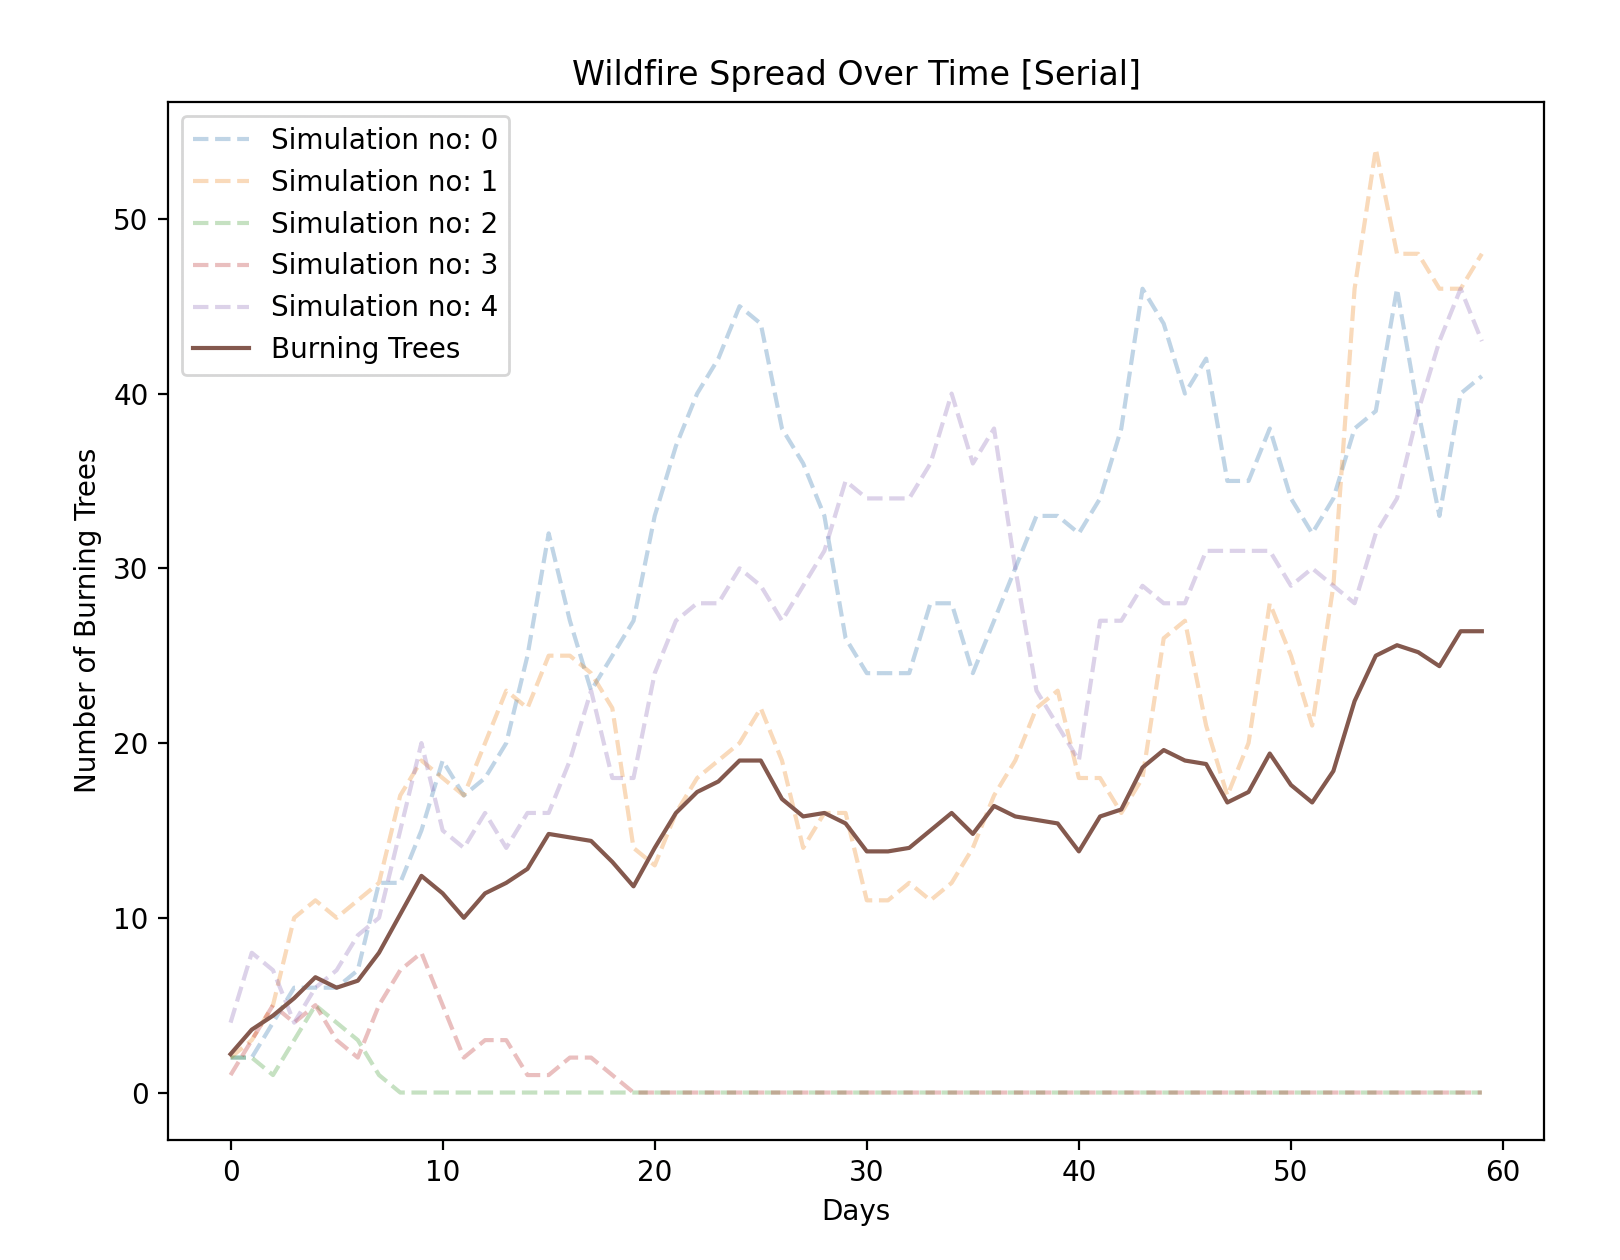
\includegraphics[width=0.8\textwidth]{../images/a4_ex1_serial_example.png}
  \caption{Average Trees Burned Per Day (Serial)}
\end{figure}


\subsection{Parallelization Using \textit{multiprocessing} Module}
The code where we parallelize using the \verb|multiprocessing| module is present in the \verb|wildfiremontecarloparallel.py| file. To summarize our implementation, we use \verb|multiprocessing.Pool| to spawn as many worker processes as we need simulations, and then use the \verb|map| function of \verb|Pool| to distribute the independent simulations across workers. We then take a column-wise mean of the result accumulated in the 2D array, converting it to a \verb|numpy| array beforehand. Thus, we return the average number of trees burned on each day based on the results for that day from the independent simulations.

With this implementation, we ran 5 simulations at once, and obtained the following line-plot. Notice that it is identical to the one obtained for the serial implementation, because of our use of seeds.


\begin{figure}[H]
  \centering
  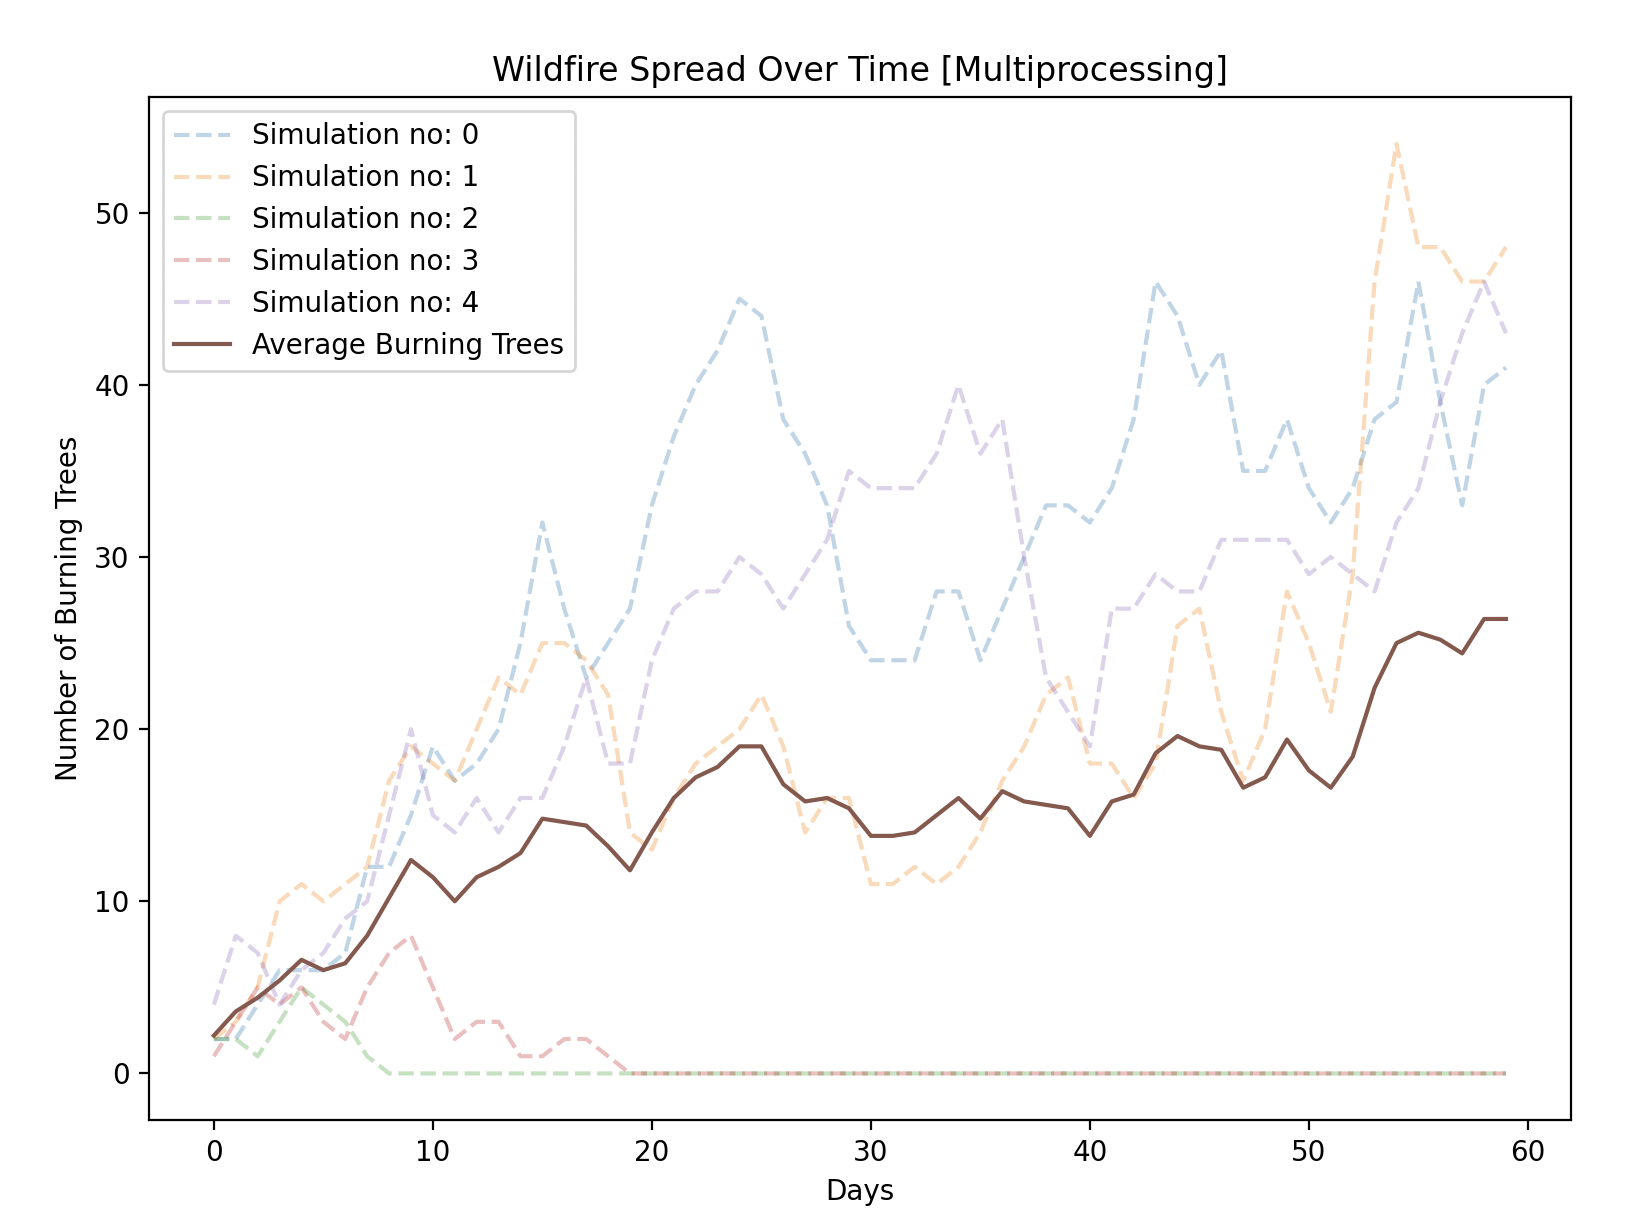
\includegraphics[width=0.8\textwidth]{../images/a4_ex1_multiprocessing_example.png}
  \caption{Average Trees Burned Per Day (Multiprocessing)}
\end{figure}

\subsection{Parallelization Using Dask}
For the Dask parallelization, we followed the steps below: 
\begin{enumerate}
\item Convert \verb|simulate_wildfire| to a Dask-Delayed function with the \verb|@delayed| annotation. We converted \verb|fire_spread| into a \verb|numpy| array before returning. This made the code for getting a dask array of the results cleaner.
\item We created an array of delayed \verb|simulate_wildfire| \textbf{tasks}, where the number of delayed tasks was equal to the numer of independend simulations required.
\item We created an intermediate array/data-structure of the delayed results (array) from the individual \verb|simulate_wildfire| tasks, using the \verb|from_delayed| function. The difference between this step and the previous one is that the former was an array of delayed \textbf{tasks}. However here, we are using the output that \textit{will} be returned from the tasks and indicating to Dask that we want them to be converted to Dask Arrays.
\item We used the \verb|stack| method of \verb|dask.array| to give the array of individual simulation results a shape that will facilitate the averaging of the number of burned trees per day.
\item We used the \verb|rechunk| operation on the result of the previous step to obtain chunks of required size. This was used to determine the impact of chunk-size (if any) on the run-time of the Dask optimization. Since the handout talked about converting the results of the simulations to a dask array, we assumed that the chunk-size impact was to be measured on this. We chunk our results array so that the averages for the days can be computed in parallel. Thus, the chunk size will have the form (\verb|num_simulations|, $x$), where $x$ is the number of days we want to assign to each chunk.
\item Finally, we average the burning trees for each day and compute the result. 
\end{enumerate}

With this implementation, we obtained the following line-plot for 5 simulations (identical to the plot for the previous 2 implementations because of seeding).

\begin{figure}[H]
  \centering
  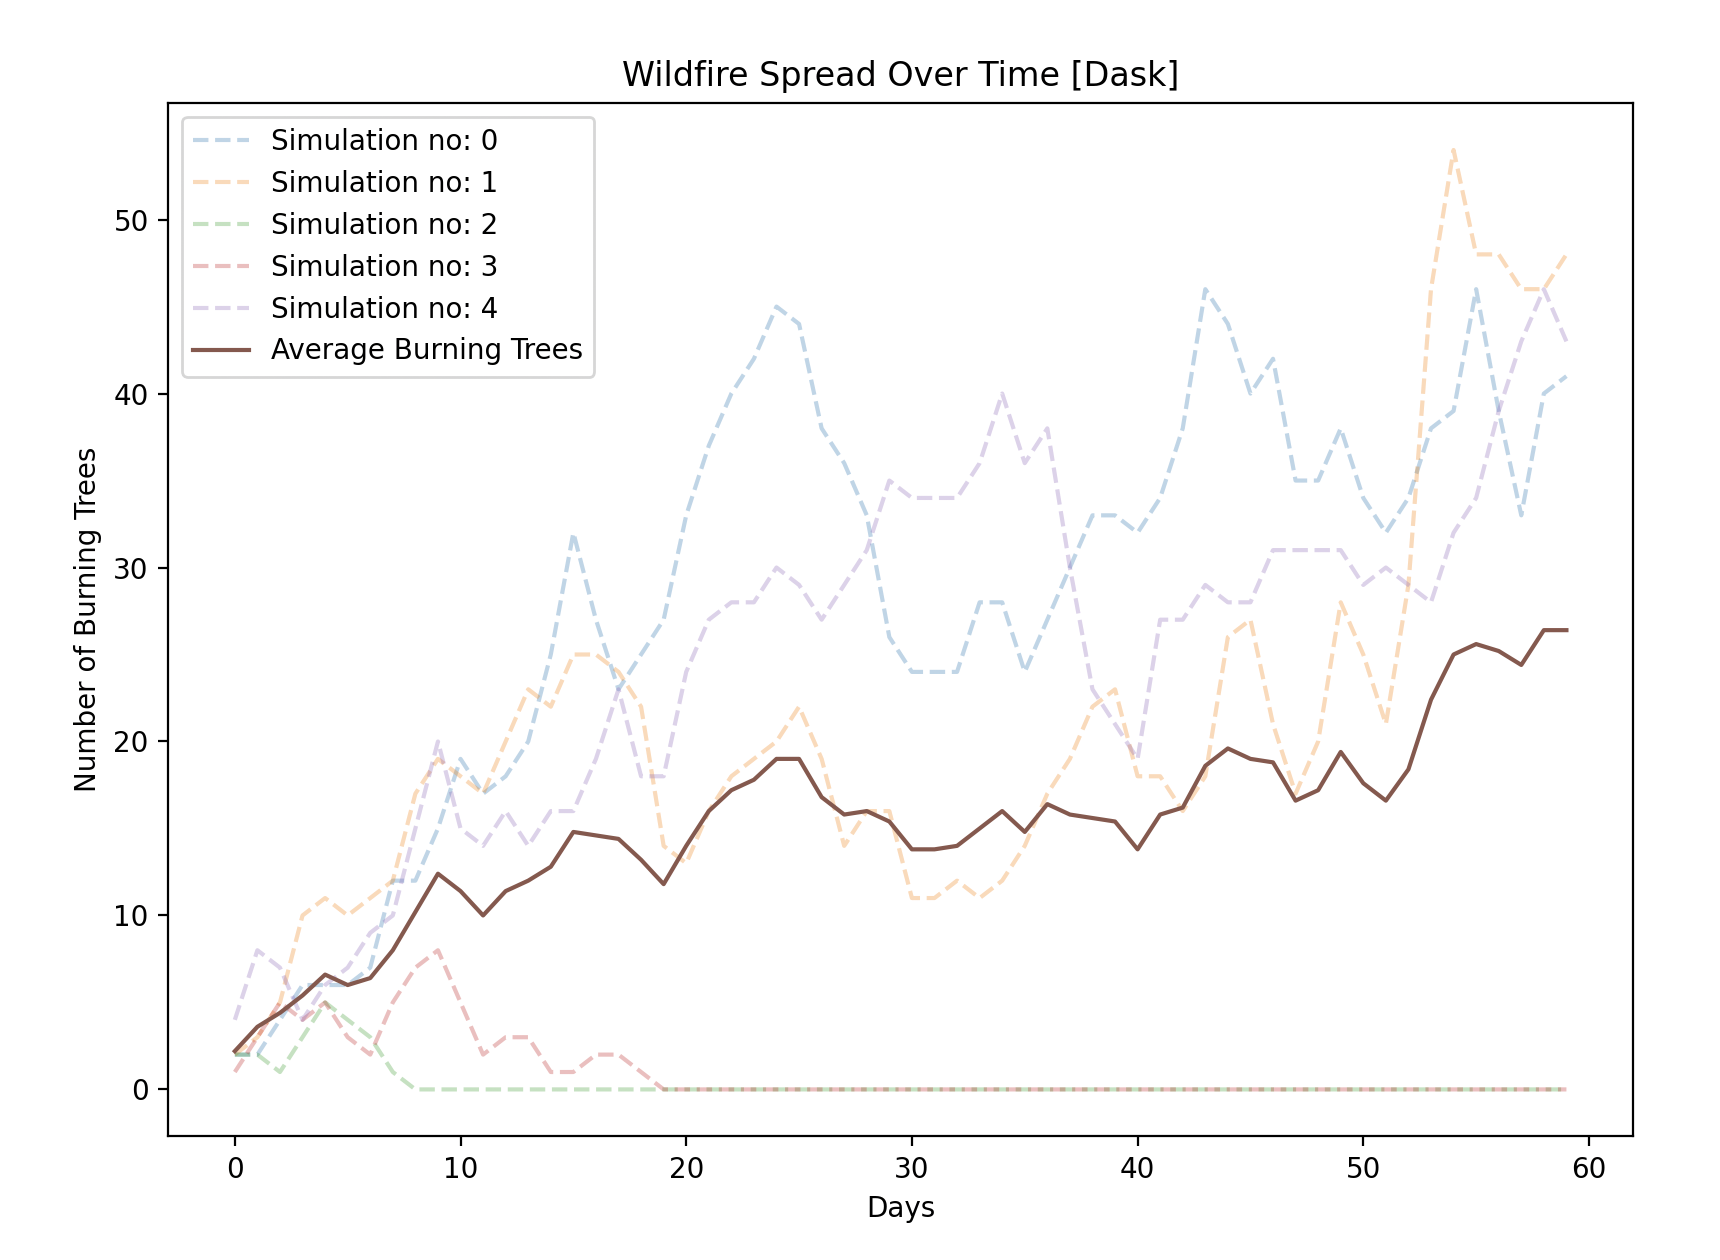
\includegraphics[width=0.8\textwidth]{../images/a4_ex1_dask_example.png}
  \caption{Average Trees Burned Per Day (Dask)}
\end{figure}

We also utilized the local \verb|Client| from \verb|dask.distributed|. We used the default configuration of the client, which on the 2021 M1 MacBook Pro (16''), was \textbf{\underline{5 workers, each with 2 threads}}. 

You can see a videos showing information from the \textbf{Status} and \textbf{Worker} Panel of the Dask Dashboard in the \verb|README.md| file for this directory at the repository, here: \href{https://github.com/paulmyr/DD2358-HPC25/tree/master/04_parallel/exercise1#readme}{link}. These recordings are from running 5 simulations at once using our Dask parallelization technique. 

The \textbf{Status} panel video (\href{https://github.com/paulmyr/DD2358-HPC25/tree/master/04_parallel/exercise1#the-status-panel}{link}) shows us the change in memory consumption, task distribution to the threads by the scheduler, and other important information at a glance. 

The \textbf{Workers} panel video (\href{https://github.com/paulmyr/DD2358-HPC25/tree/master/04_parallel/exercise1#the-workers-panel}{link}) shows us information about CPU usage and memory usage for each worker. Here, we can see that the workers seem to be busy (at almost 100\% CPU capacity) most of the time, which indicates that Dask Scheduler did a \textbf{reasonably good} job of allocating jobs to the workers in this run. Most of the work seems to be done during the \verb|from_delayed| computation, as the blue rectangles seem to refer to a \verb|from-value| call, which we assume to be that method. 

Below, we also attach a screenshot of the \textbf{Task Stream} Panel during a 5-simulation run, where we can see the task distribution across the 10 threads more easily. In this run, it seems that 3 threads had a minimal amount of work to do, as there are almost no rectangles allocated to them. 

\begin{figure}[H]
  \centering
  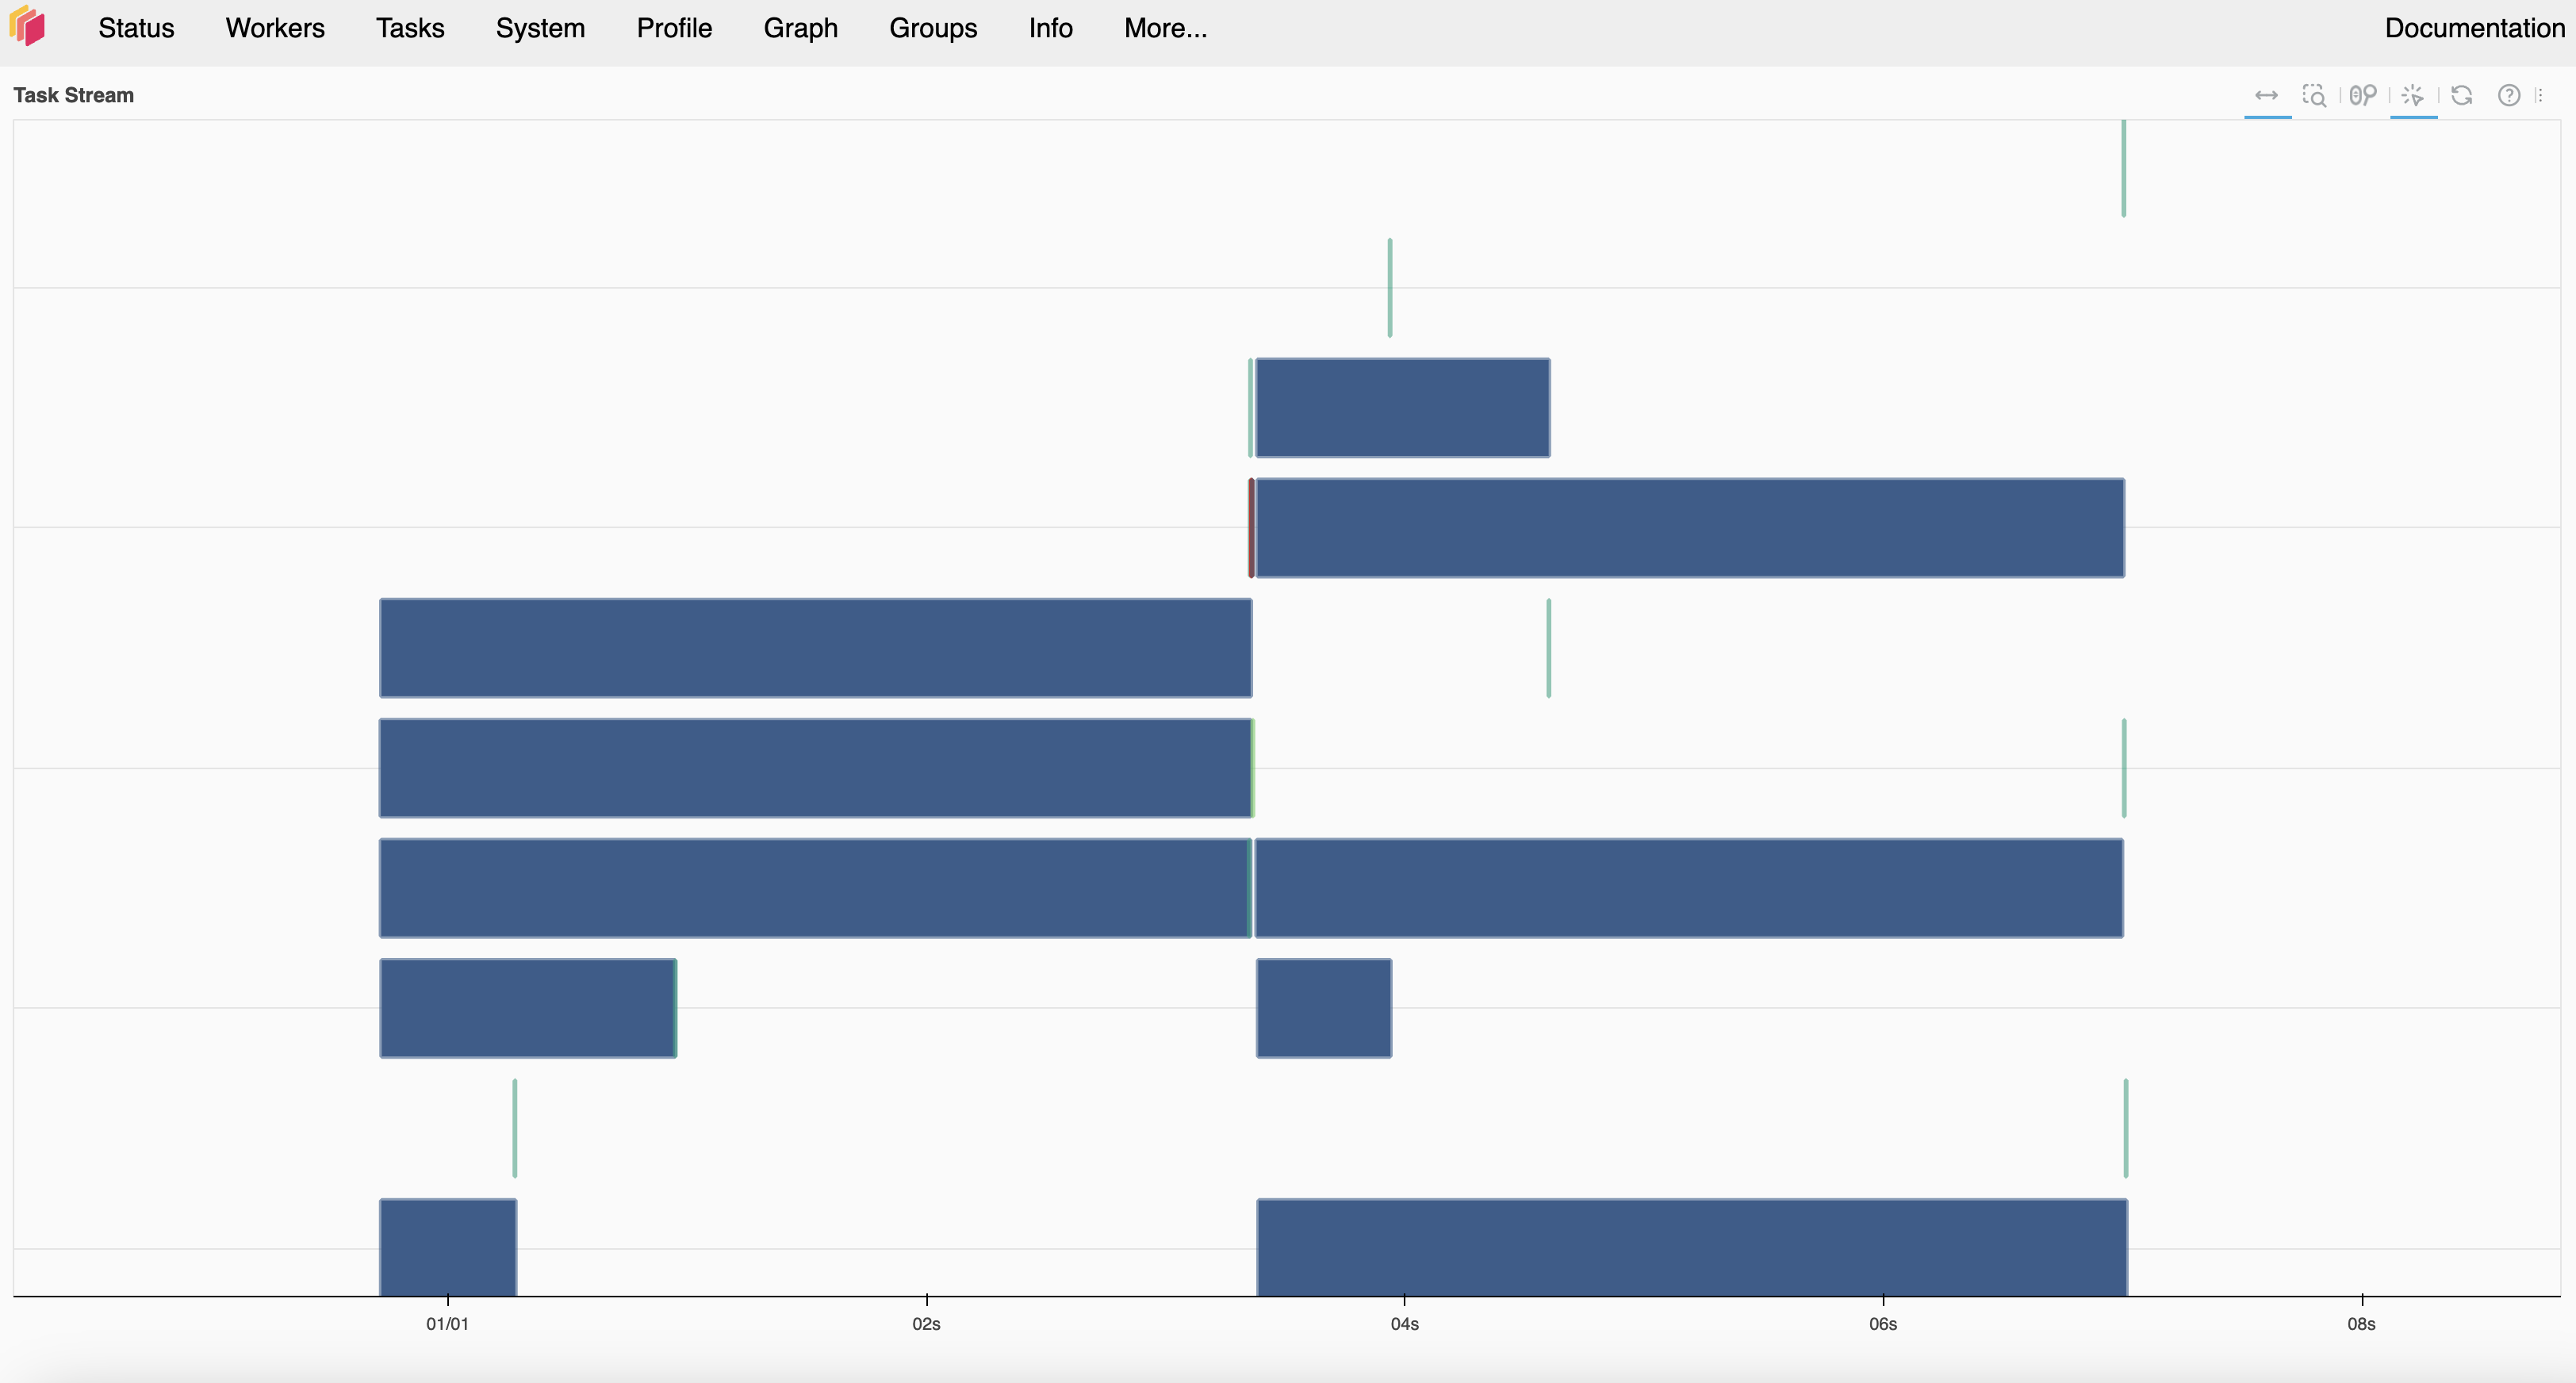
\includegraphics[width=0.8\textwidth]{../images/a4_ex1_dask_task_stream.png}
  \caption{Task Stream for 5 Simulations}
\end{figure}

\subsection*{Note: Correctness Verification of Parallel Approaches}
The \verb|wildfire_test.py| file contains some parameterized-tests that ensure that the averages returned for certain number of simulations by the \verb|multiprocessing| and \verb|Dask| parallelization techniques match the output returned by the \verb|serial| technique. We use seeding to ensure reproducability of the results. All these tests pass.

\subsection{Performance Comparison \& Questions}

\subsubsection{Performance Comparison}
The plot below shows the execution time of the 3 implementations for different number of simulations. 
\begin{figure}[H]
  \centering
  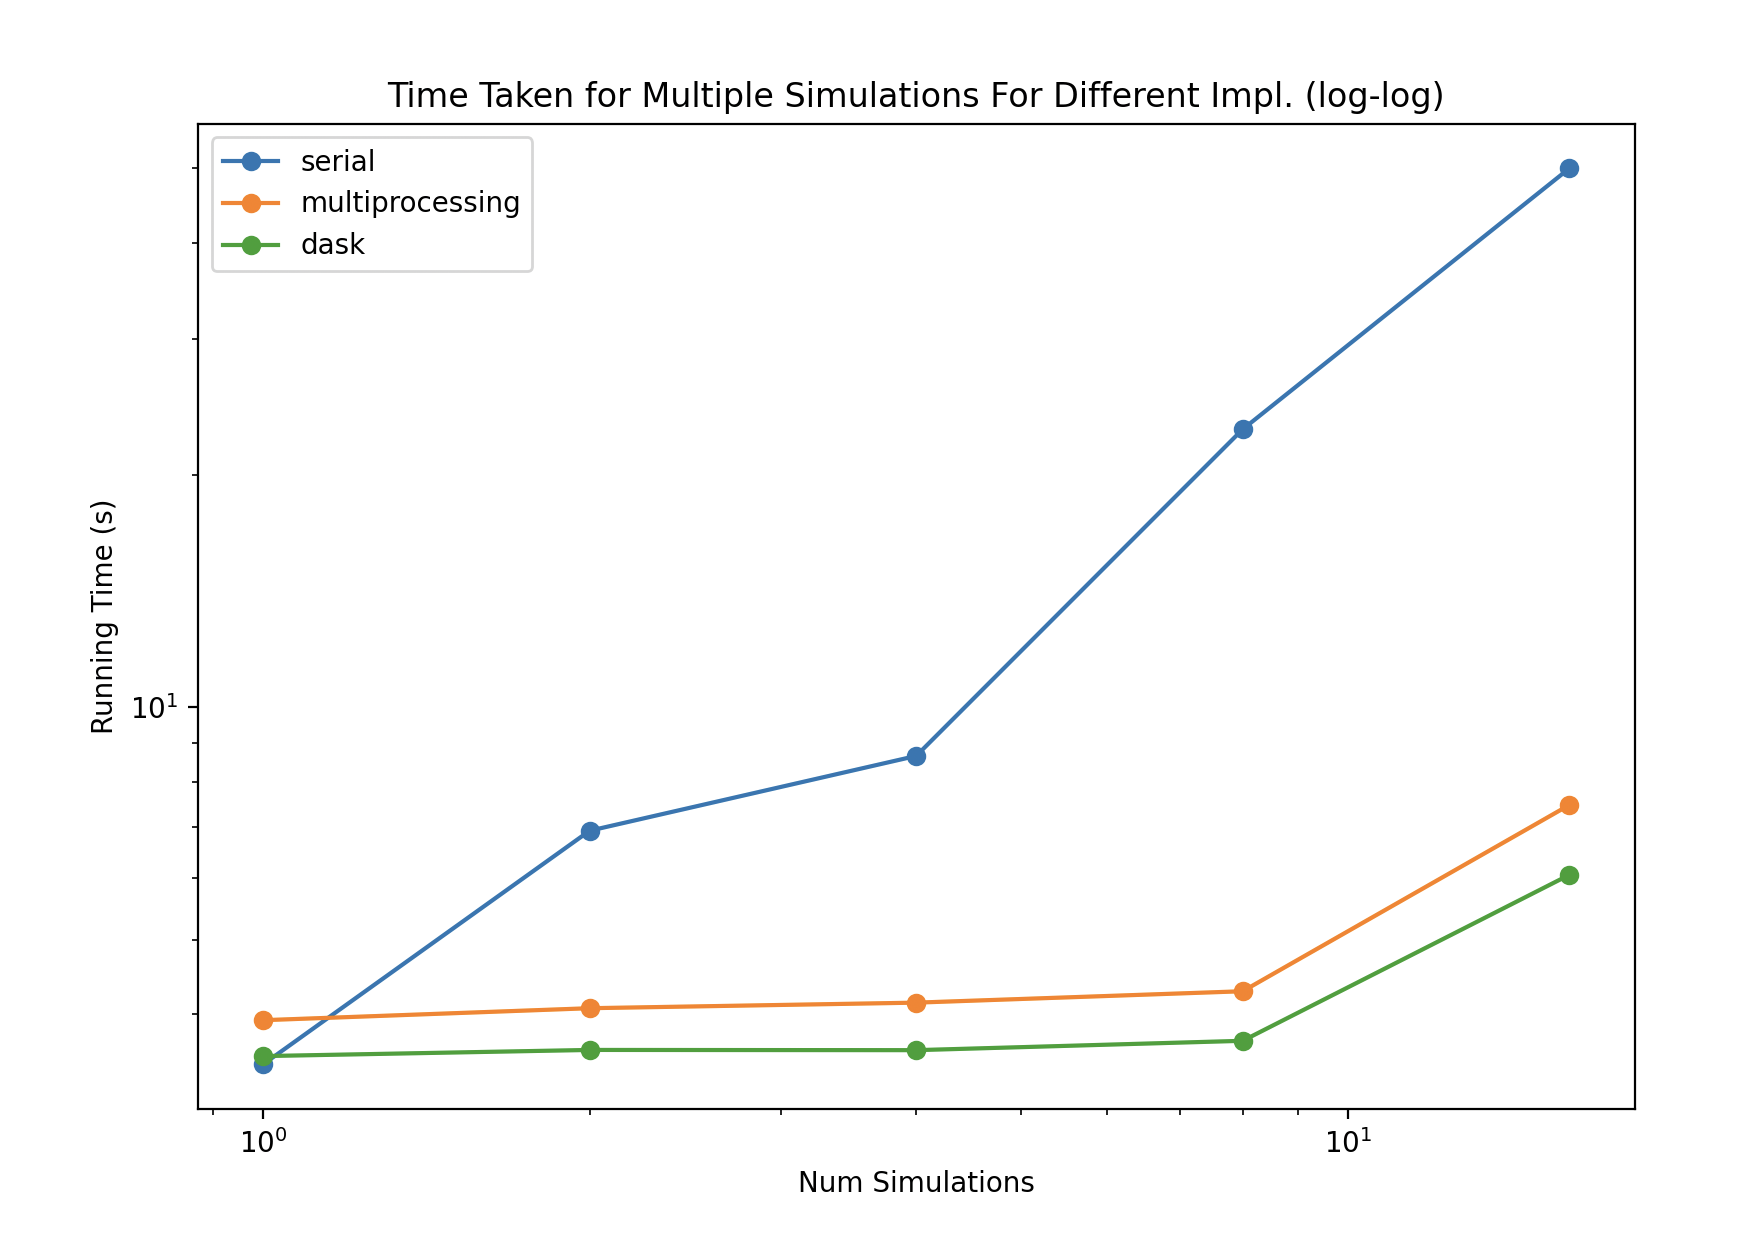
\includegraphics[width=0.6\textwidth]{../images/a4_ex1_runtime_comparison.png}
  \caption{Execution Time Comparison of the 3 Approaches}
\end{figure}

Below you can see the textual output visualized in the plot above:

\begin{lstlisting}[language=bash,basicstyle=\tiny\ttfamily]
$ sudo python3 wildfire_profile.py
PROFILING COMPUTATION FOR serial IMPLEMENTATION (runs=3)
Avg Time for 1 simulations: 3.445551611002884 s 
Avg Time for 2 simulations: 6.9186229303353075 s 
Avg Time for 4 simulations: 8.648581541667227 s 
Avg Time for 8 simulations: 22.92307461099699 s 
Avg Time for 16 simulations: 49.92087736133059 s 
PROFILING COMPUTATION FOR multiprocessing IMPLEMENTATION (runs=3)
Avg Time for 1 simulations: 3.9312227636692114 s 
Avg Time for 2 simulations: 4.07437822233381 s 
Avg Time for 4 simulations: 4.142661333661333 s 
Avg Time for 8 simulations: 4.285970041664162 s 
Avg Time for 16 simulations: 7.470850749998742 s 
PROFILING COMPUTATION FOR dask IMPLEMENTATION (runs=3)
Avg Time for 1 simulations: 3.5319369026692584 s 
Avg Time for 2 simulations: 3.5974722913330575 s 
Avg Time for 4 simulations: 3.5950862220003423 s 
Avg Time for 8 simulations: 3.6969253473265176 s 
Avg Time for 16 simulations: 6.064963166335171 s 
\end{lstlisting}

For Dask, we used \textbf{as many workers as number of simulations (1 thread per worker)}. The code for this can be found in the \verb|wildfire_profile.py| file. \textit{Note: On the laptop with specifications defined above, we had to increase the \textbf{ulimit} on the command line to get 16 workers in this and any profiling that follows. Without this, we got \textbf{Too Many Files Open} exceptions, similar to this SO thread: \href{https://stackoverflow.com/questions/18280612/ioerror-errno-24-too-many-open-files}{link}}. 

The number of simulations are powers of 2 in the range of $1\dots16$. From the figure, it is clear that \textbf{both parallel approaches outperform the serial approach}. For 1 simulation, the serial approach is slightly better. This makes sense to us, as the cost of setting up the \verb|multiprocessing|/Dask overhead would make it difficult to see any performance gain for a single simulation. However, as we increase the number of simulations, the serial approach can only execute 1 independent simulation at a time, while \verb|multiprocessing| and Dask then seem to gain advantage of multipple parallel executions. 

Overall, \textbf{Dask seems to outperform the other approaches}. Note that for both the parallel approaches, the runtime seems to be unchanged up until 8 simulations. However, as soon as we jump to 16 simulations, there is a noticeable increase in the runtime. We believe that this can be attributed to the fact that we are trying to run \textbf{more parallel jobs than cores available} on the machine. As mentioned above, the setup has 10 cores. Thus, running 16 simulations in parallel using 16 processes or workers is impossible. Thus, there seems to be some contention to run on the 10 cores available, which likely explains the pattern observed here.

\subsubsection{Which version is the fastest?}
As examined above, the \textbf{Dask approach} seems to be the fastest.

\subsubsection{How well does Dask scale with different number of workers?}
We compared the running time for running 8 and 16 simulations as the number of workers increase from $2 \rightarrow 4 \rightarrow 8 \rightarrow 16$ (with 1 thread per worker). The code for this can be found in the \verb|worker_profile.py| file. On doing so, we obtained the following plot
\begin{figure}[H]
  \centering
  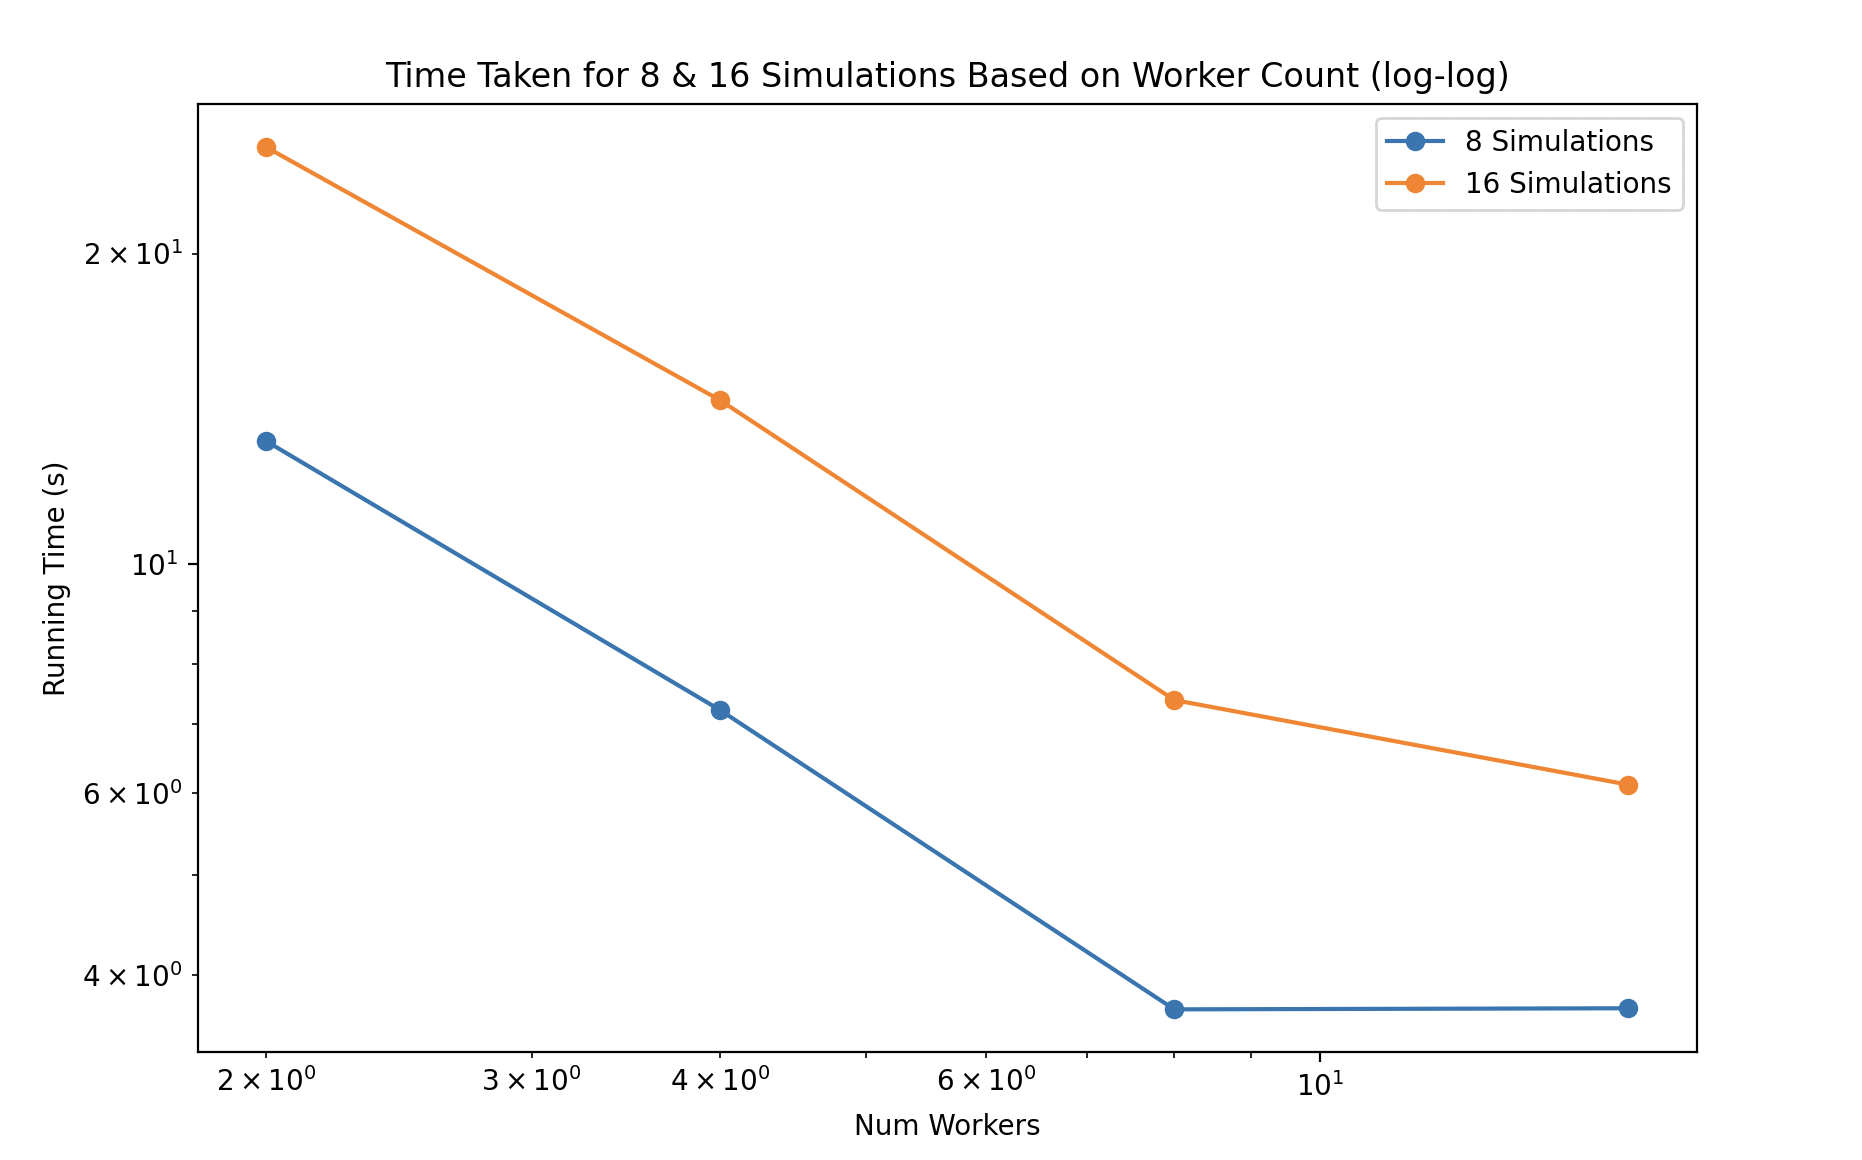
\includegraphics[width=0.6\textwidth]{../images/a4_ex1_worker_comparison.png}
  \caption{Impact of \#Workers on Dask Parallel Simulations}
\end{figure}

Below you can see the textual output that is being visualized in the plot above:
\begin{lstlisting}[language=bash,basicstyle=\tiny\ttfamily]
$ python3 worker_profile.py
PROFILING COMPUTATION FOR DASK IMPLEMENTATION (runs=3, workers=2)
Avg Time for 8 simulations: 13.164127069331395 s 
Avg Time for 16 simulations: 25.36850654166483 s 
PROFILING COMPUTATION FOR DASK IMPLEMENTATION (runs=3, workers=4)
Avg Time for 8 simulations: 7.221452972332675 s 
Avg Time for 16 simulations: 14.417073847662929 s 
PROFILING COMPUTATION FOR DASK IMPLEMENTATION (runs=3, workers=8)
Avg Time for 8 simulations: 3.7034622503318437 s 
Avg Time for 16 simulations: 7.384757389004032 s 
PROFILING COMPUTATION FOR DASK IMPLEMENTATION (runs=3, workers=16)
Avg Time for 8 simulations: 3.7125208473347207 s 
Avg Time for 16 simulations: 6.11314287466909 s
\end{lstlisting}

In general, the pattern seems to be that an \textbf{increase in the number of workers reduces the running time}. This is in line with our expectations. On the plot, it is interesting to see that there is a sharp decline in the runtime up until 8 workers -- likely because all 8 workers can work in parallel on the 10 available cores. However, the rate at which the runtime declines for 16 workers is not as steep. 

For 8 simulations, this could be because increasing the number of workers beyond the number of parallel simulations would just mean that some workers end up doing nothing, and so it has minimal effect. However, for the 16 simulations case, this could point to the limitations in the amount of parallelism that can be achieved when we have more workers than available cores. Even then, there does seem to be a slight decline in runtime for the 16 workers -- 16 simulations combination. 

So, increasing workers (assuming they all have 1 thread) seems to be one easy way of improving performance for Dask, and thus Dask seems to \textbf{scale well} with the number of workers. 

\subsubsection{How does chunk size affect performance?}
To examine the impact of chunk size in the computation of the average on the final dask-array for the 60 days across simulations, we \textbf{varied the number of days} that are allocated to each chunk when computing the averages. The chunk sizes varied from $10 \rightarrow 20 \rightarrow 30 \rightarrow 60$ days. We ran a constant 8 simulations with this setup, using the default configuration of \verb|Client| on our machine, with \textbf{\underline{5 workers and 2 threads per worker}}. The code for this can be found in the \verb|chunk_profile.py| file. 

With this setup, we obtained the following plot of the runtime when varying the chunk-sizes: 
\begin{figure}[H]
  \centering
  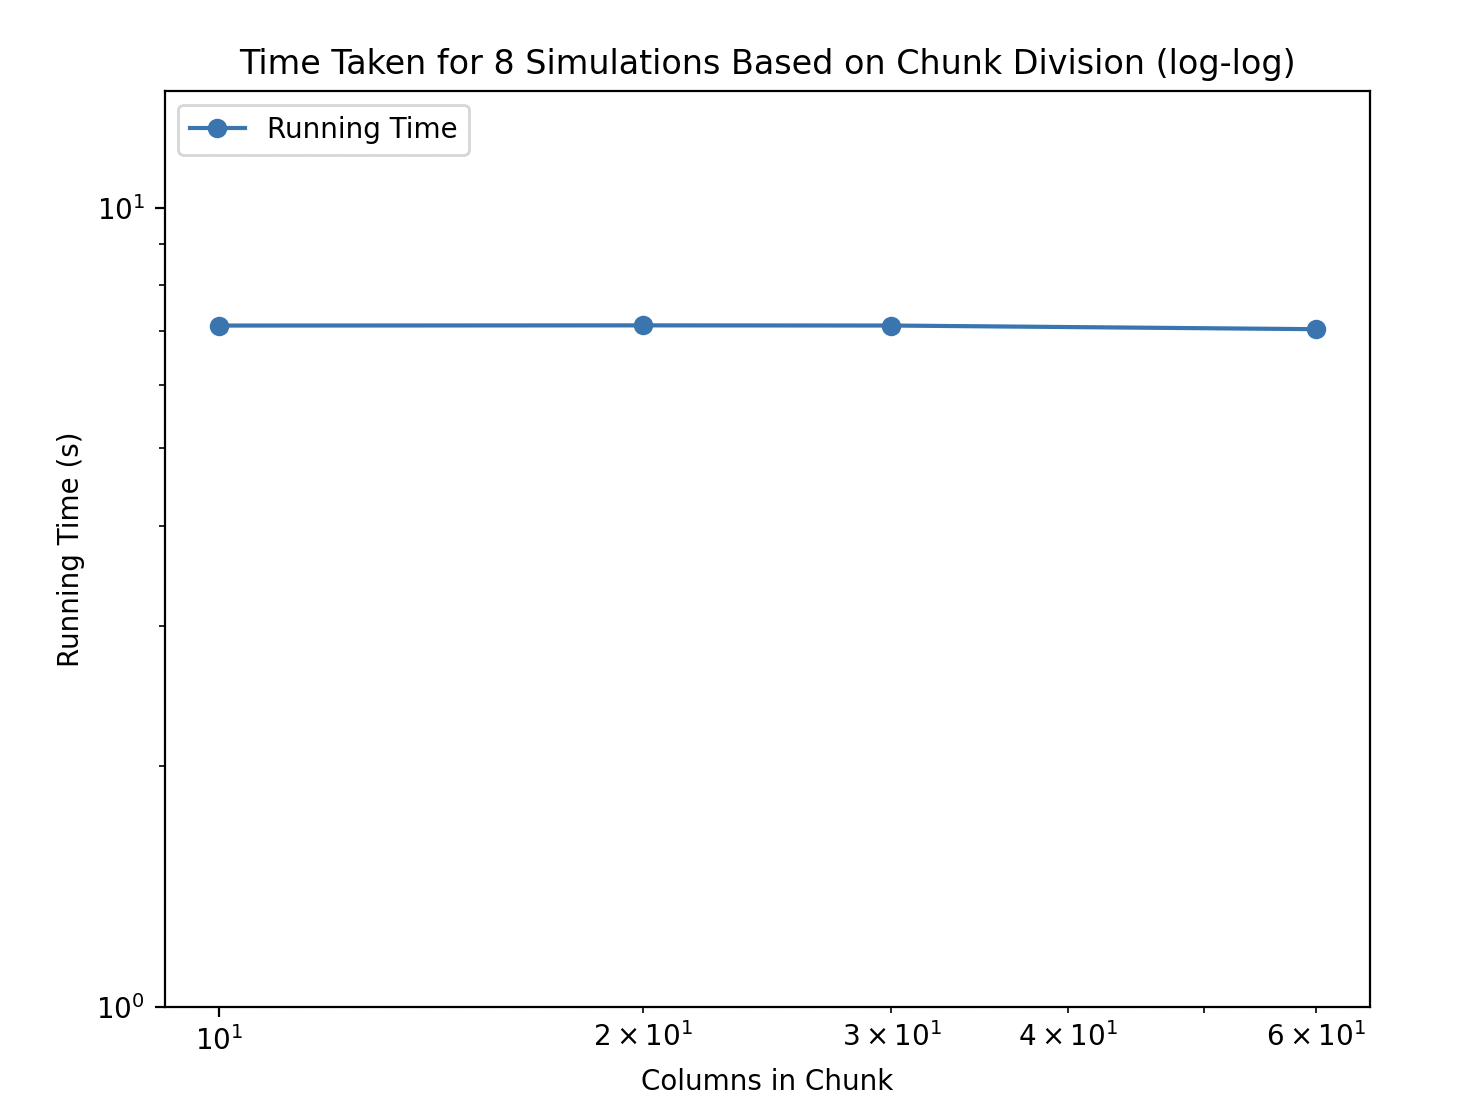
\includegraphics[width=0.6\textwidth]{../images/a4_ex1_chunks.png}
  \caption{Impact of Chunk Sizes on Dask Parallel Simulations}
\end{figure}

Below you can see the textual output that is being visualized in the plot above:
\begin{lstlisting}[language=bash,basicstyle=\tiny\ttfamily]
$ python3 chunk_profile.py
PROFILING COMPUTATION FOR DASK IMPLEMENTATION (runs=3, chunk_columns=10)
Avg Time for 8 simulations: 7.120227680667692 s 
PROFILING COMPUTATION FOR DASK IMPLEMENTATION (runs=3, chunk_columns=20)
Avg Time for 8 simulations: 7.124035903000428 s 
PROFILING COMPUTATION FOR DASK IMPLEMENTATION (runs=3, chunk_columns=30)
Avg Time for 8 simulations: 7.120728333335137 s 
PROFILING COMPUTATION FOR DASK IMPLEMENTATION (runs=3, chunk_columns=60)
Avg Time for 8 simulations: 7.04620731966376 s
\end{lstlisting}

In all cases, the chunk size has \textbf{\underline{minimal impact}} on the runtime of the Dask implementation. All these runtimes are incredibly similar, with the fastest one being when we have 1 chunk (ie, when \verb|chunk_columns=60|). Even then, the runtime seems close enough to the other cases for it to not be of high significance. This is similar to our expectations -- as we feel that the final Dask array we are working with (with 8 simulations) to not be big enough to have any noticeable performance improvements with chunking. 

We believe that we will start seeing noticeable differences when it comes to chunking when the final array over which the average is computed gets big enough such that chunk-size determines whether or not that array is able to fit in to the processor cache. However, up until 128 simulations (which would give us a $128 \times 60$ result grid over which the average is computed), the chunk size did not seem to impact runtime on our setup. 

Thus, we believe that \textbf{chunk size has minimal impact on execution time} up to atleast 100 simulations being run in parallel using Dask on our setup

\subsection{VTK Visualization of the Grid}
The code in \verb|wildfiremontecarloserial.py| file was augmented to allow for saving the state of the \verb|forest| to vtk file every few time-steps. The function \verb|save_data_to_vtk| is responsible for creating and saving this VTK data. To get a more comprehensive visualization, the \verb|DAYS| parameter in the file was changed to 500 from 60 (it has been changed back afterwards). Note that only the data obtained from the serial implementation was saved to VTK in this way, as was clarified in the Canvas discussion (\href{https://canvas.kth.se/courses/52247/discussion_topics/453192}{link}). The VTK files so generated can be found under the \verb|vtk/| subdirectory of the \verb|exercise1/| directory for this assignment.

You can find the entire animation from Paraview in the \verb|README.md| for this subdirectory in the repo, at this location: \href{https://github.com/paulmyr/DD2358-HPC25/blob/master/04_parallel/exercise1/README.md#the-vtk-visualization-on-paraview}{link}.

Here, we attach 5 screenshots from the animation, taken at an interval of 25 time steps (including the first and last frame).

\begin{figure}
\centering
\begin{subfigure}{0.4\textwidth}
    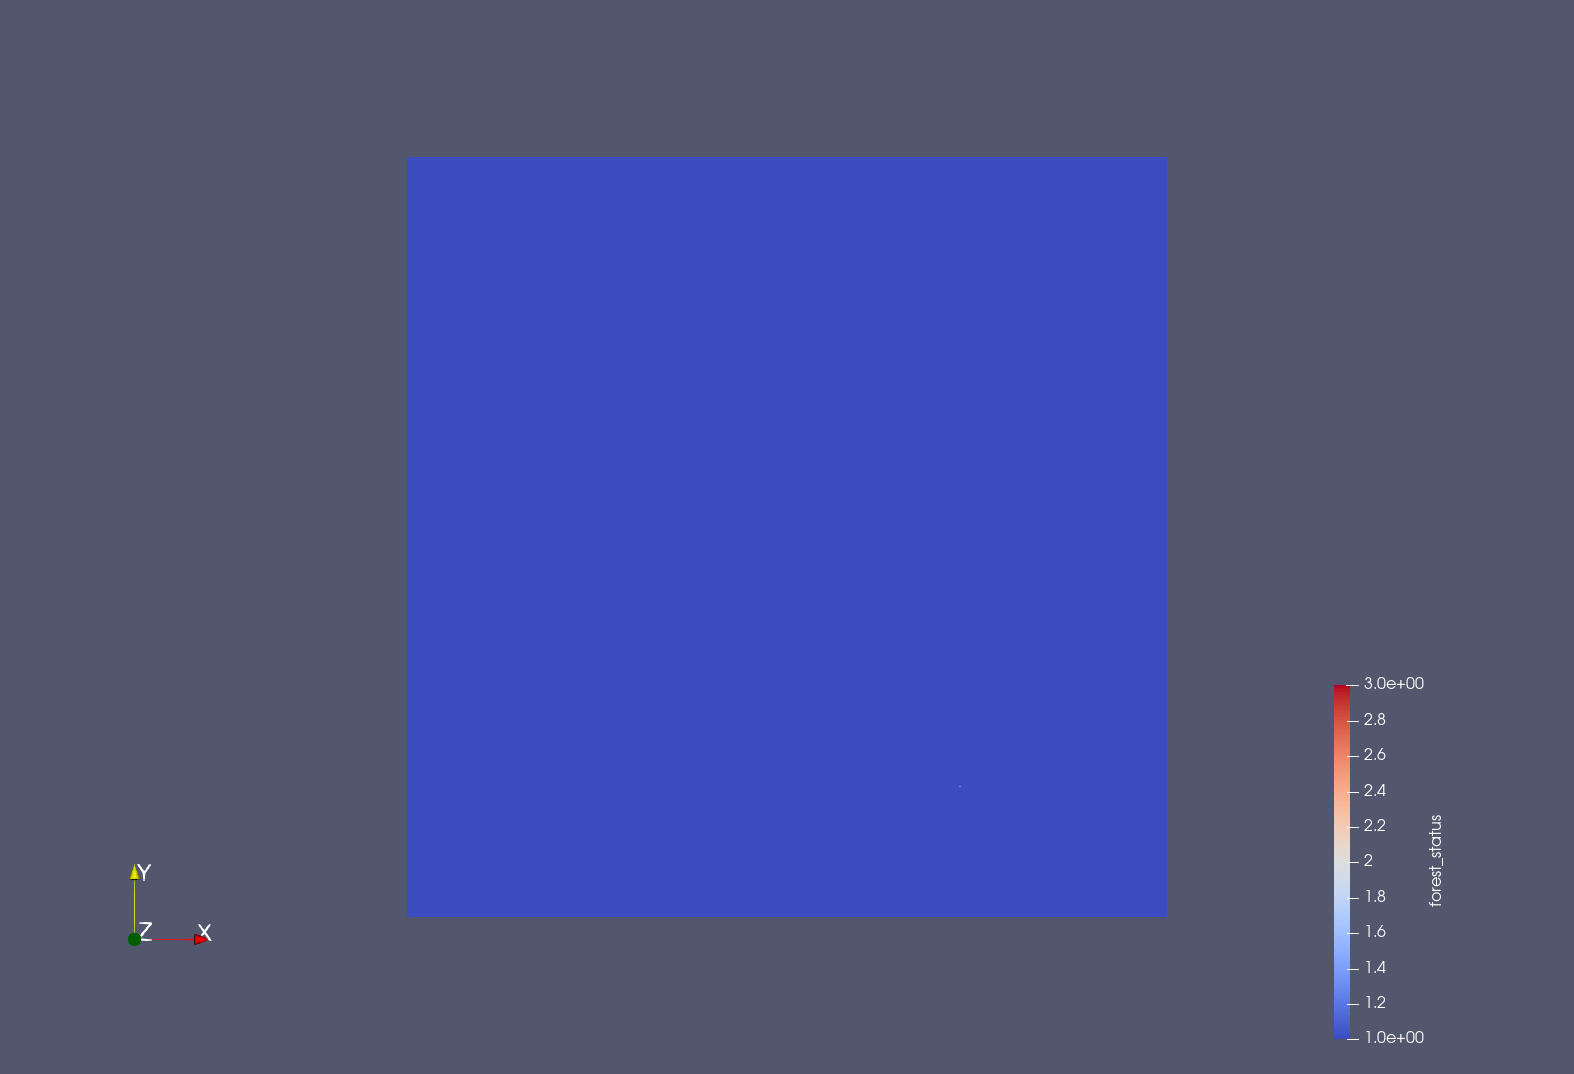
\includegraphics[width=\textwidth]{../images/vtk/ex1/step_0.png}
    \caption{Step 0}
\end{subfigure}
\hfill
\begin{subfigure}{0.4\textwidth}
    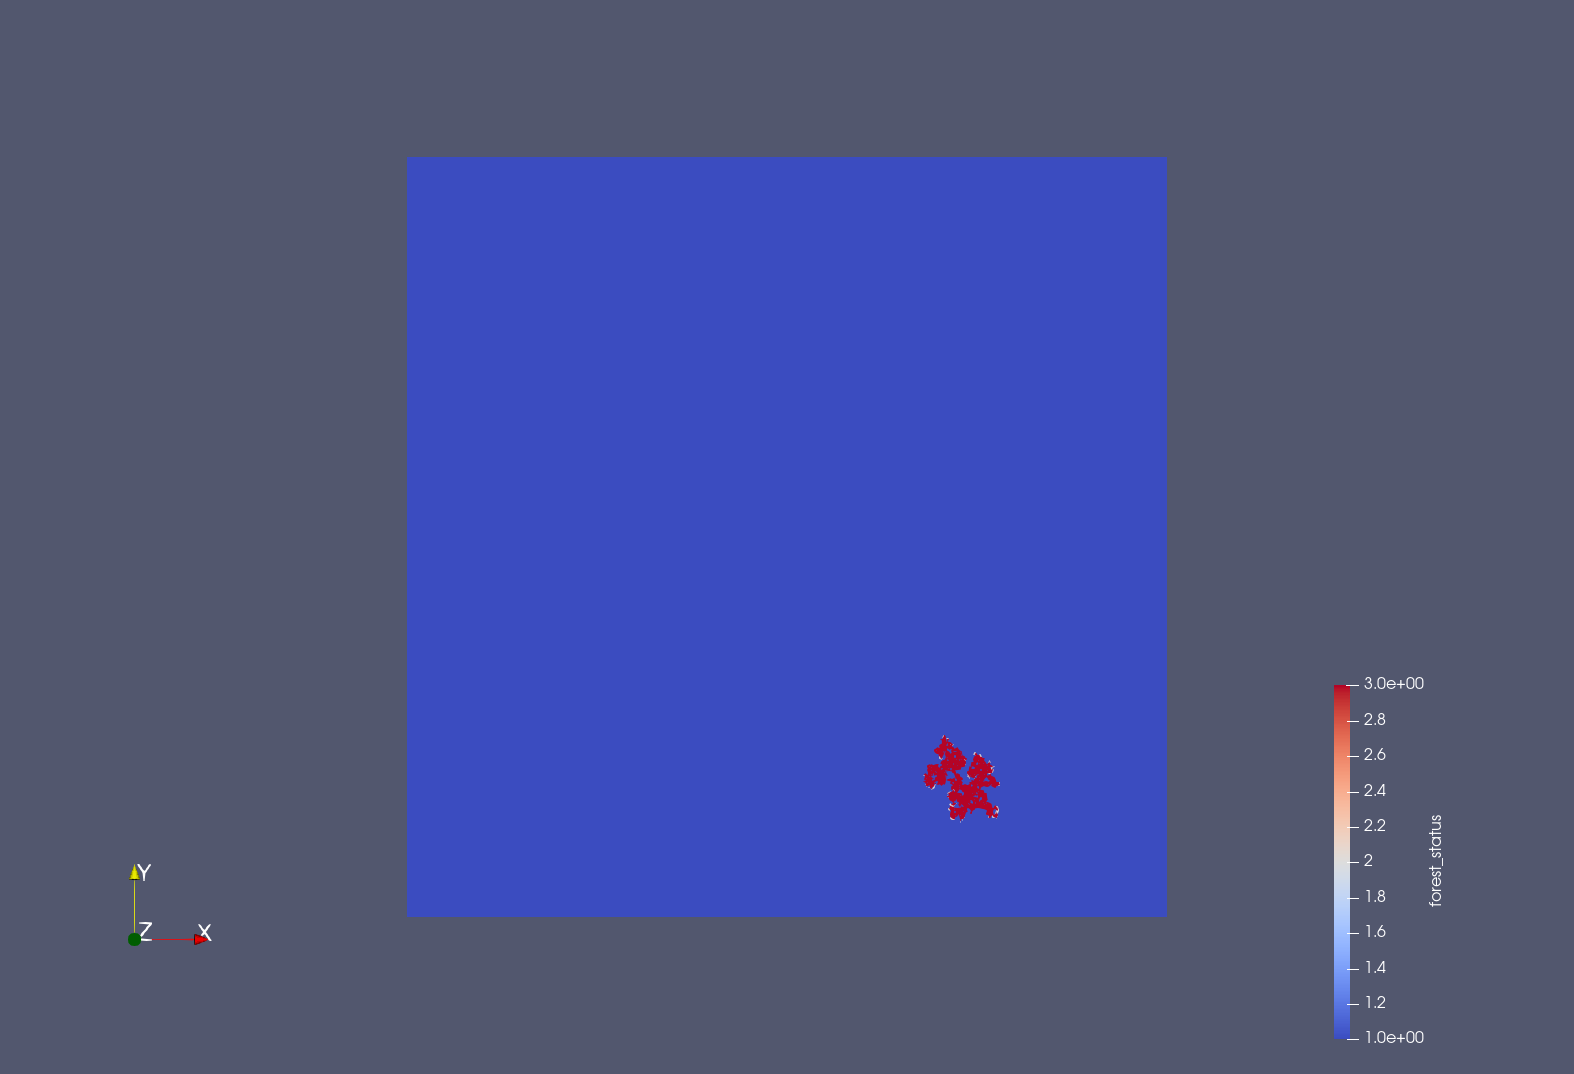
\includegraphics[width=\textwidth]{../images/vtk/ex1/step_25.png}
    \caption{Step 25}
\end{subfigure}
\hfill
\begin{subfigure}{0.4\textwidth}
    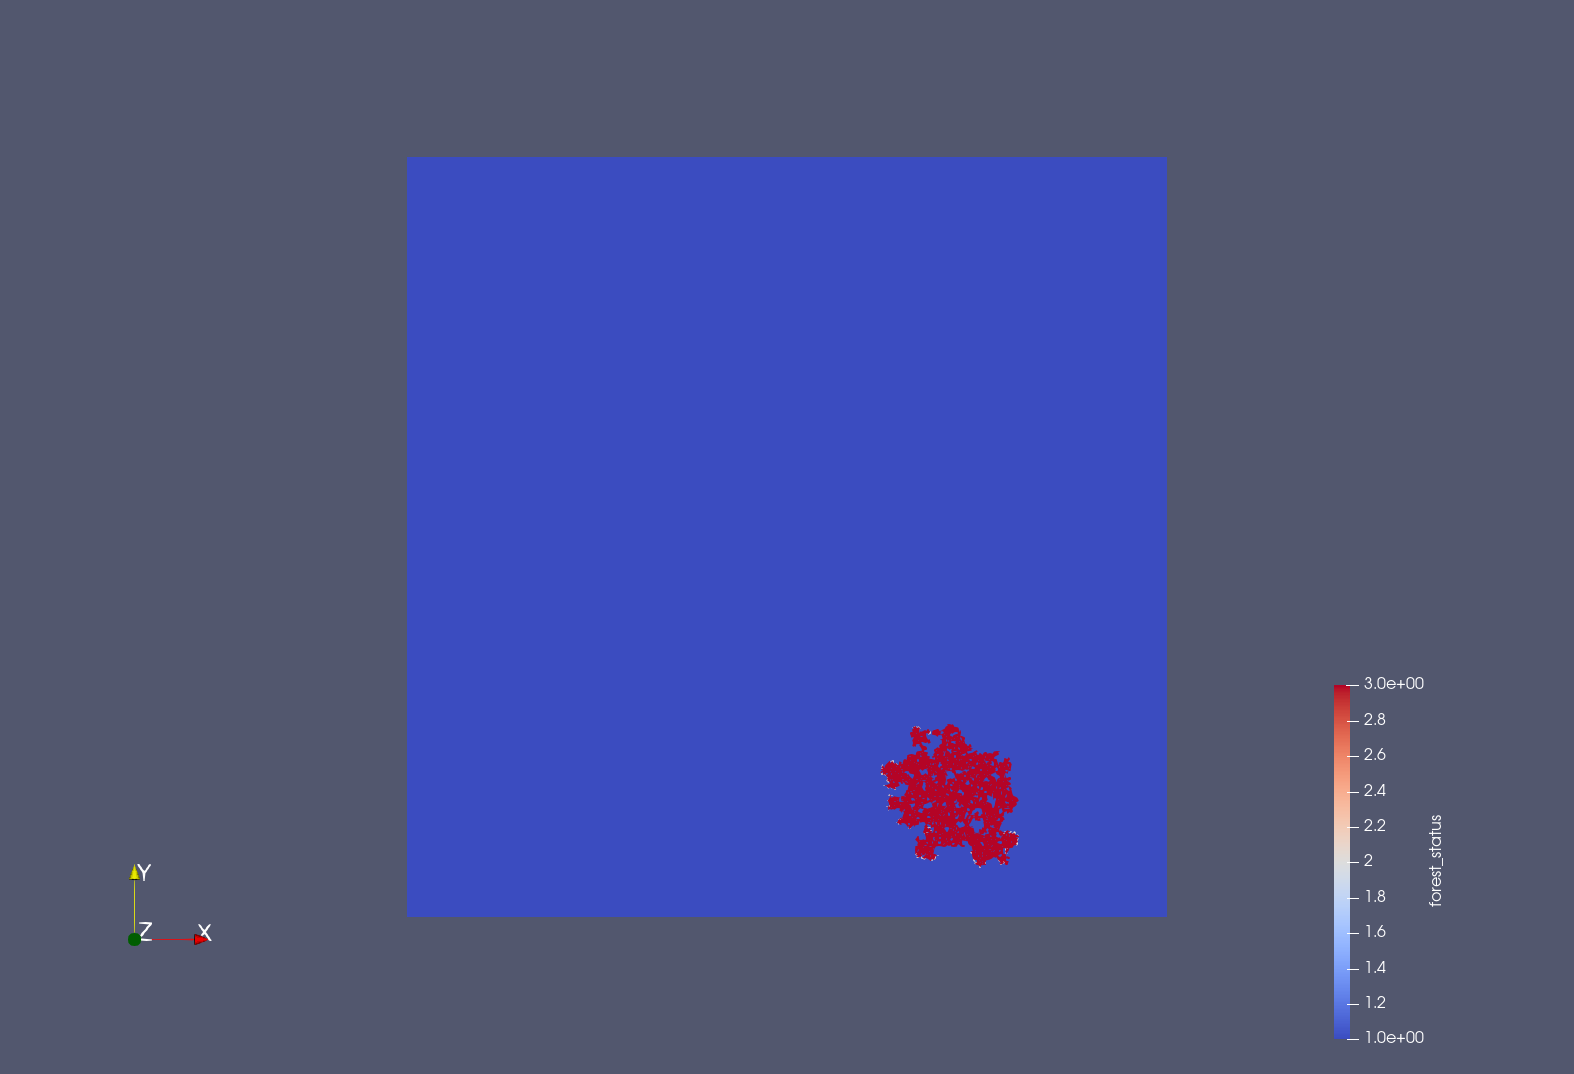
\includegraphics[width=\textwidth]{../images/vtk/ex1/step_50.png}
    \caption{Step 50}
\end{subfigure}
\hfill
\begin{subfigure}{0.4\textwidth}
    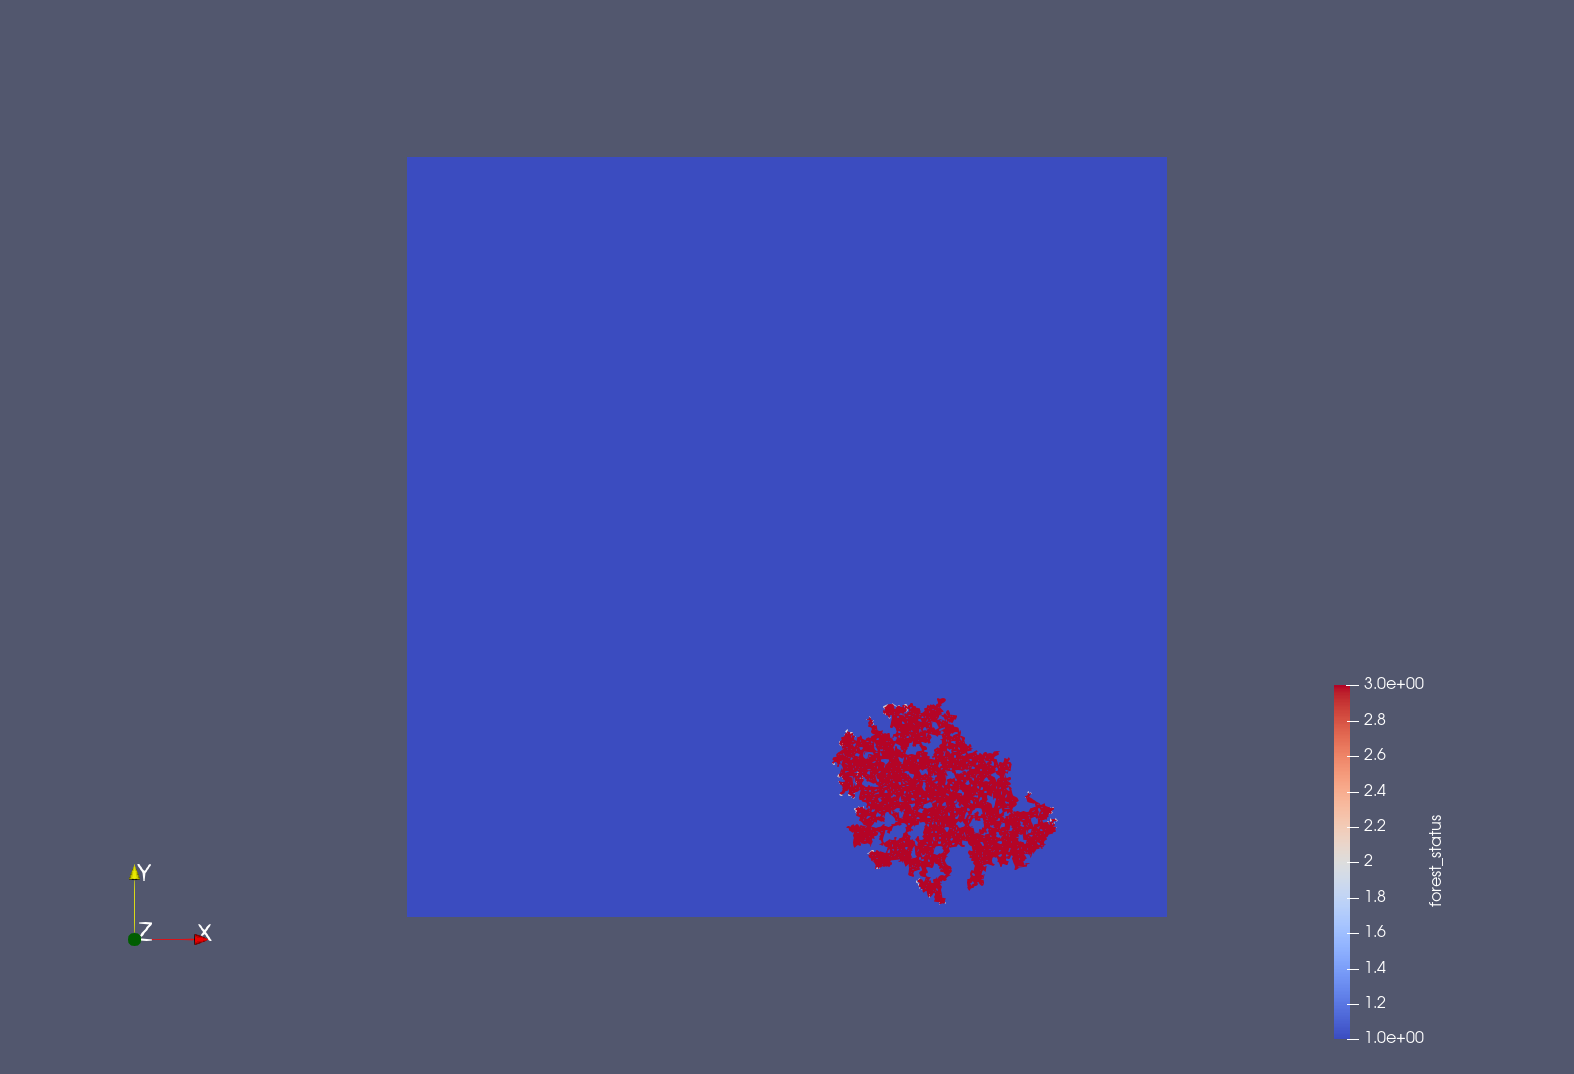
\includegraphics[width=\textwidth]{../images/vtk/ex1/step_75.png}
    \caption{Step 75}
\end{subfigure}

\begin{subfigure}{0.4\textwidth}
    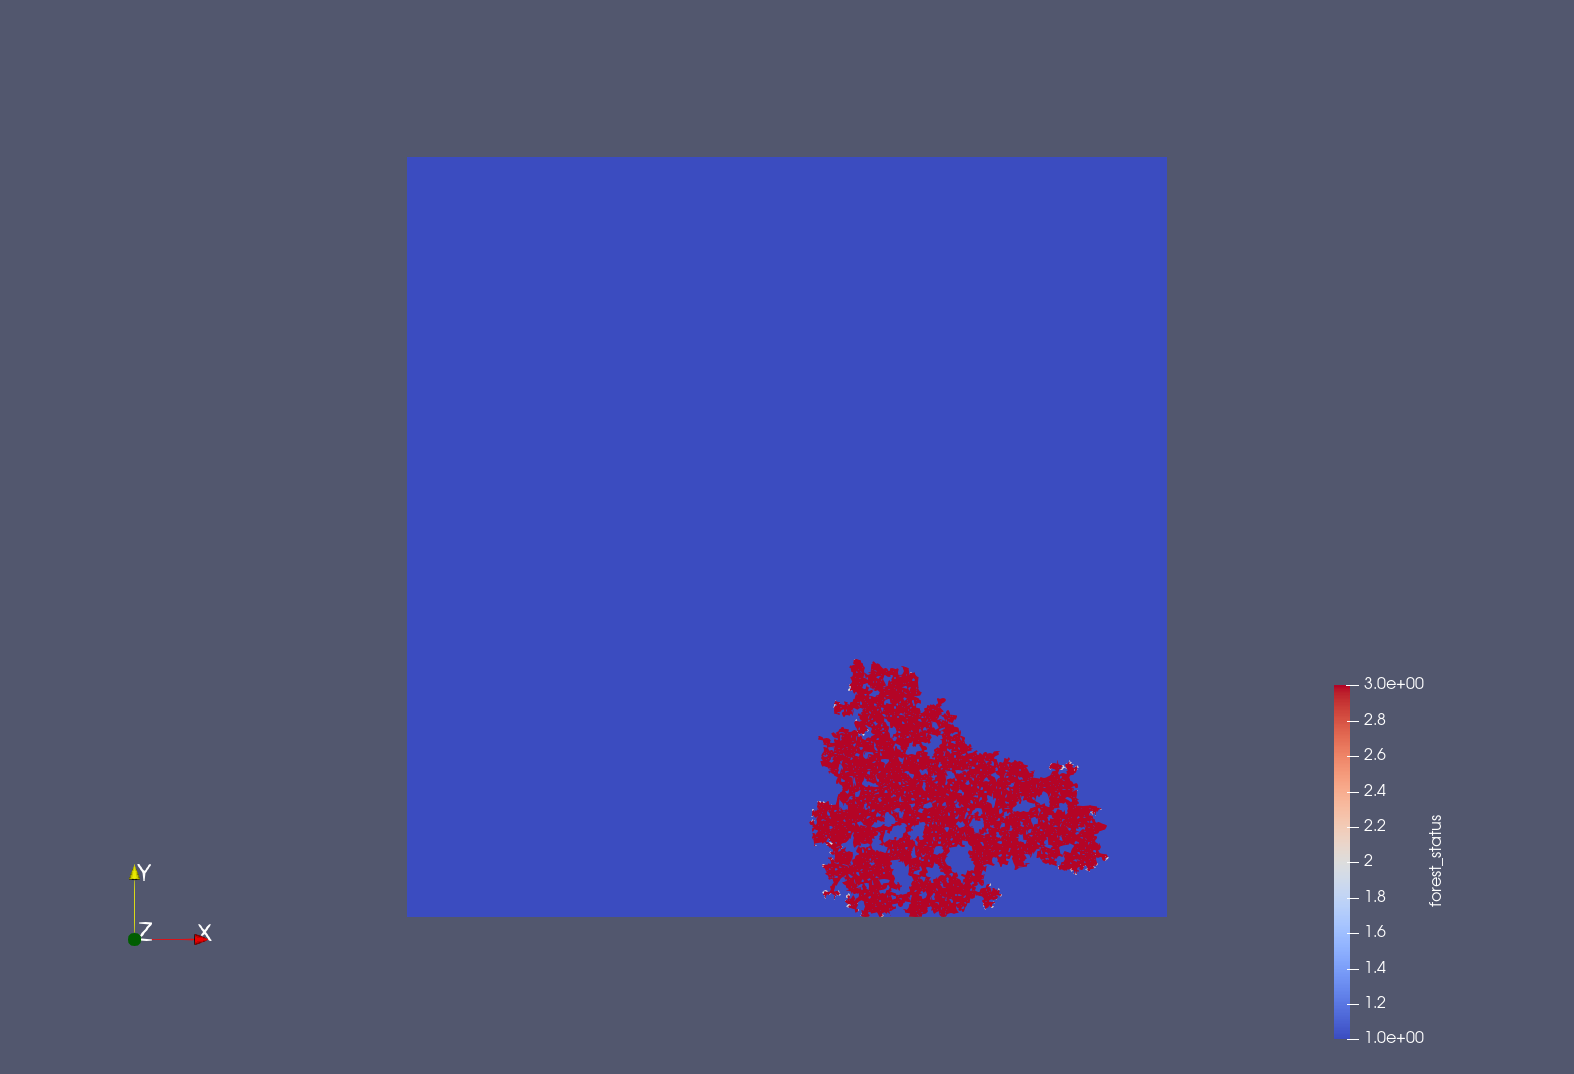
\includegraphics[width=\textwidth]{../images/vtk/ex1/step_100.png}
    \caption{Step 100}
\end{subfigure}

\caption{Screenshots from Paraview Forest Fire Visualization}
\end{figure}


\section{Bonus: Ocean Circulation with Dask}
The code and associated files for the bonus section can be found under the \verb|bonus/| directory of the repository, here: \url{https://github.com/paulmyr/DD2358-HPC25/tree/master/04_parallel/bonus}. The original code provided to us can be found in the \verb|ocean_deafult.py| file -- with some augmentation to help with profiling and testing against the Dask implementation. The observations made, including the screenshots and video recordings, were obtained on a 2021 M1 MacBook Pro (16 inch), the specifications for which can be found \href{https://support.apple.com/en-us/111901}{here}.

\subsection{Dask Implementation}

\subsubsection{Brief Explanation}
To parallelize the provided code with Dask, we utilized the \verb|map_overlap| function of the Dask arrays to \textit{schedule} the parallel updates to our 3 arrays -- \verb|u_velocity|, \verb|v_velocity|, and \verb|temperature|. The Dask-parallelized implementation can be found in the \verb|ocean_dask.py| file in the repository.

We first converted all the grids used in the ocean updates from \verb|numpy| arrays to Dask arrays using the \verb|da.from_array| function with a specified chunk size (in the report, \verb|da| refers to \verb|dask.array|). 

For clarity: we created two separate \verb|update| functions for the changes to the velocity and temperature grids.
We passed in these functions as the first argument to \verb|map_overlap|.
This was followed by the arguments of the \verb|update| functions.
The \verb|depth| argument of the \verb|map_overlap| function was set to 1, since that is all that was required in the overalpping computation performed by the laplacian calculation through the \verb|np.roll| operation.
Lastly, \verb|boundary| was set to be \verb|periodic|.
It gives the intended output when compared with the default serial implementation.

All in all, the overlay in \verb|ocean_dask.py| looks like this:

\begin{lstlisting}[language=python,basicstyle=\tiny\ttfamily]
# ... other code
        u_velocity = da.map_overlap(update_velocity, u_velocity, wind, depth=1, boundary="periodic", dtype=da.float64)
        v_velocity = da.map_overlap(update_velocity, v_velocity, wind, depth=1, boundary="periodic", dtype=da.float64)
        temperature = da.map_overlap(update_temp, temperature, depth=1, boundary="periodic", dtype=da.float64)
# ... other code

\end{lstlisting}

Dask then builds a \textit{task graph} which applies the updates (and the laplacian operation that is required to perform the updates) to grid partitions in parallel, instead of working on entire grids in one go.
This is performed in a loop for the desired number of iterations. 

However, due to lazy computations \textit{nothing is computed here}.
Dask only builds a computation task graph at this point (as explained in this \href{https://canvas.kth.se/courses/52247/discussion_topics/452810}{Canvas announcement}).
To get the actual \textit{result} of the computations, we call the \verb|compute()| function on the \verb|u_velocity|, \verb|v_velocity|, and \verb|temperature| Dask arrays \textbf{\underline{after}} the loop, and then return the result.
See \verb|ocean_dask.py| for the complete implementation.

\subsubsection{Correctness Verification}
To ensure that the Dask implementation returns the same result as the default, we implemented some sanity-checks in the form of unit tests.
They can be found in the \verb|ocean_test.py| file.
These are parameterized tests that run the ocean update simulations for 3 different numbers, testing that the Dask implementation returns the correct answer for 3 different chunk sizes.
We set the same seed in the Dask and the default implementation to ensure that the starting grids are the same. 

\subsubsection{Runtime Comparison}
We compared the running times of the default implementation against the Dask implementation with different chunk-sizes ($50 \times 50, 100 \times 100, 200 \times 200$). The code for this time profiling can be found in the \verb|ocean_profile.py| file. 

We compared the running times of four versions of the simulation, where each version was run for 100, 200, 400, and 800 iterations.
For each run, the runtime recorded was an average over five runs.
For the default python implementation, only the running time of the \verb|for| loop was recorded.
For the Dask implementation, the running time of the \verb|for| loop (where the task graph is created) and of the three compute calls on the Dask arrays (where the actual computation is performed) was recorded.
The code demarcating which portion of the simulation was timed can be found in the \verb|ocean_default.py| and the \verb|ocean_dask.py| files, in the \verb|run_simulation_default| and the \verb|run_simulation_dask| functions, respectively.

With this setup, we observed the following running times textual format: 

\begin{lstlisting}[language=bash,basicstyle=\tiny\ttfamily]
$ python3 ocean_profile.py
PROFILING COMPUTATION FOR DEFAULT IMPLEMENTATION (runs=5)
Avg Time for 100 iterations: 0.034803566599293845 s 
Avg Time for 200 iterations: 0.06937524999957531 s 
Avg Time for 400 iterations: 0.13857185839951852 s 
Avg Time for 800 iterations: 0.27716657480050344 s 
PROFILING COMPUTATION FOR DASK IMPLEMENTATION (chunk_size=50, runs=5)
Avg Time for 100 iterations: 6.83086175799981 s 
Avg Time for 200 iterations: 14.691950425000687 s 
Avg Time for 400 iterations: 32.8788943749998 s 
Avg Time for 800 iterations: 77.39897956659988 s 
PROFILING COMPUTATION FOR DASK IMPLEMENTATION (chunk_size=100, runs=5)
Avg Time for 100 iterations: 2.7626196668003105 s 
Avg Time for 200 iterations: 6.482563008401485 s 
Avg Time for 400 iterations: 15.559239650000382 s 
Avg Time for 800 iterations: 41.137253450201385 s 
PROFILING COMPUTATION FOR DASK IMPLEMENTATION (chunk_size=200, runs=5)
Avg Time for 100 iterations: 1.6673615167994285 s 
Avg Time for 200 iterations: 3.9416711081998073 s 
Avg Time for 400 iterations: 10.363534933399205 s 
Avg Time for 800 iterations: 30.311092333000126 s 
$
\end{lstlisting}

And this is a graph which visualizes the same values recorded above

\begin{figure}[H]
  \centering
  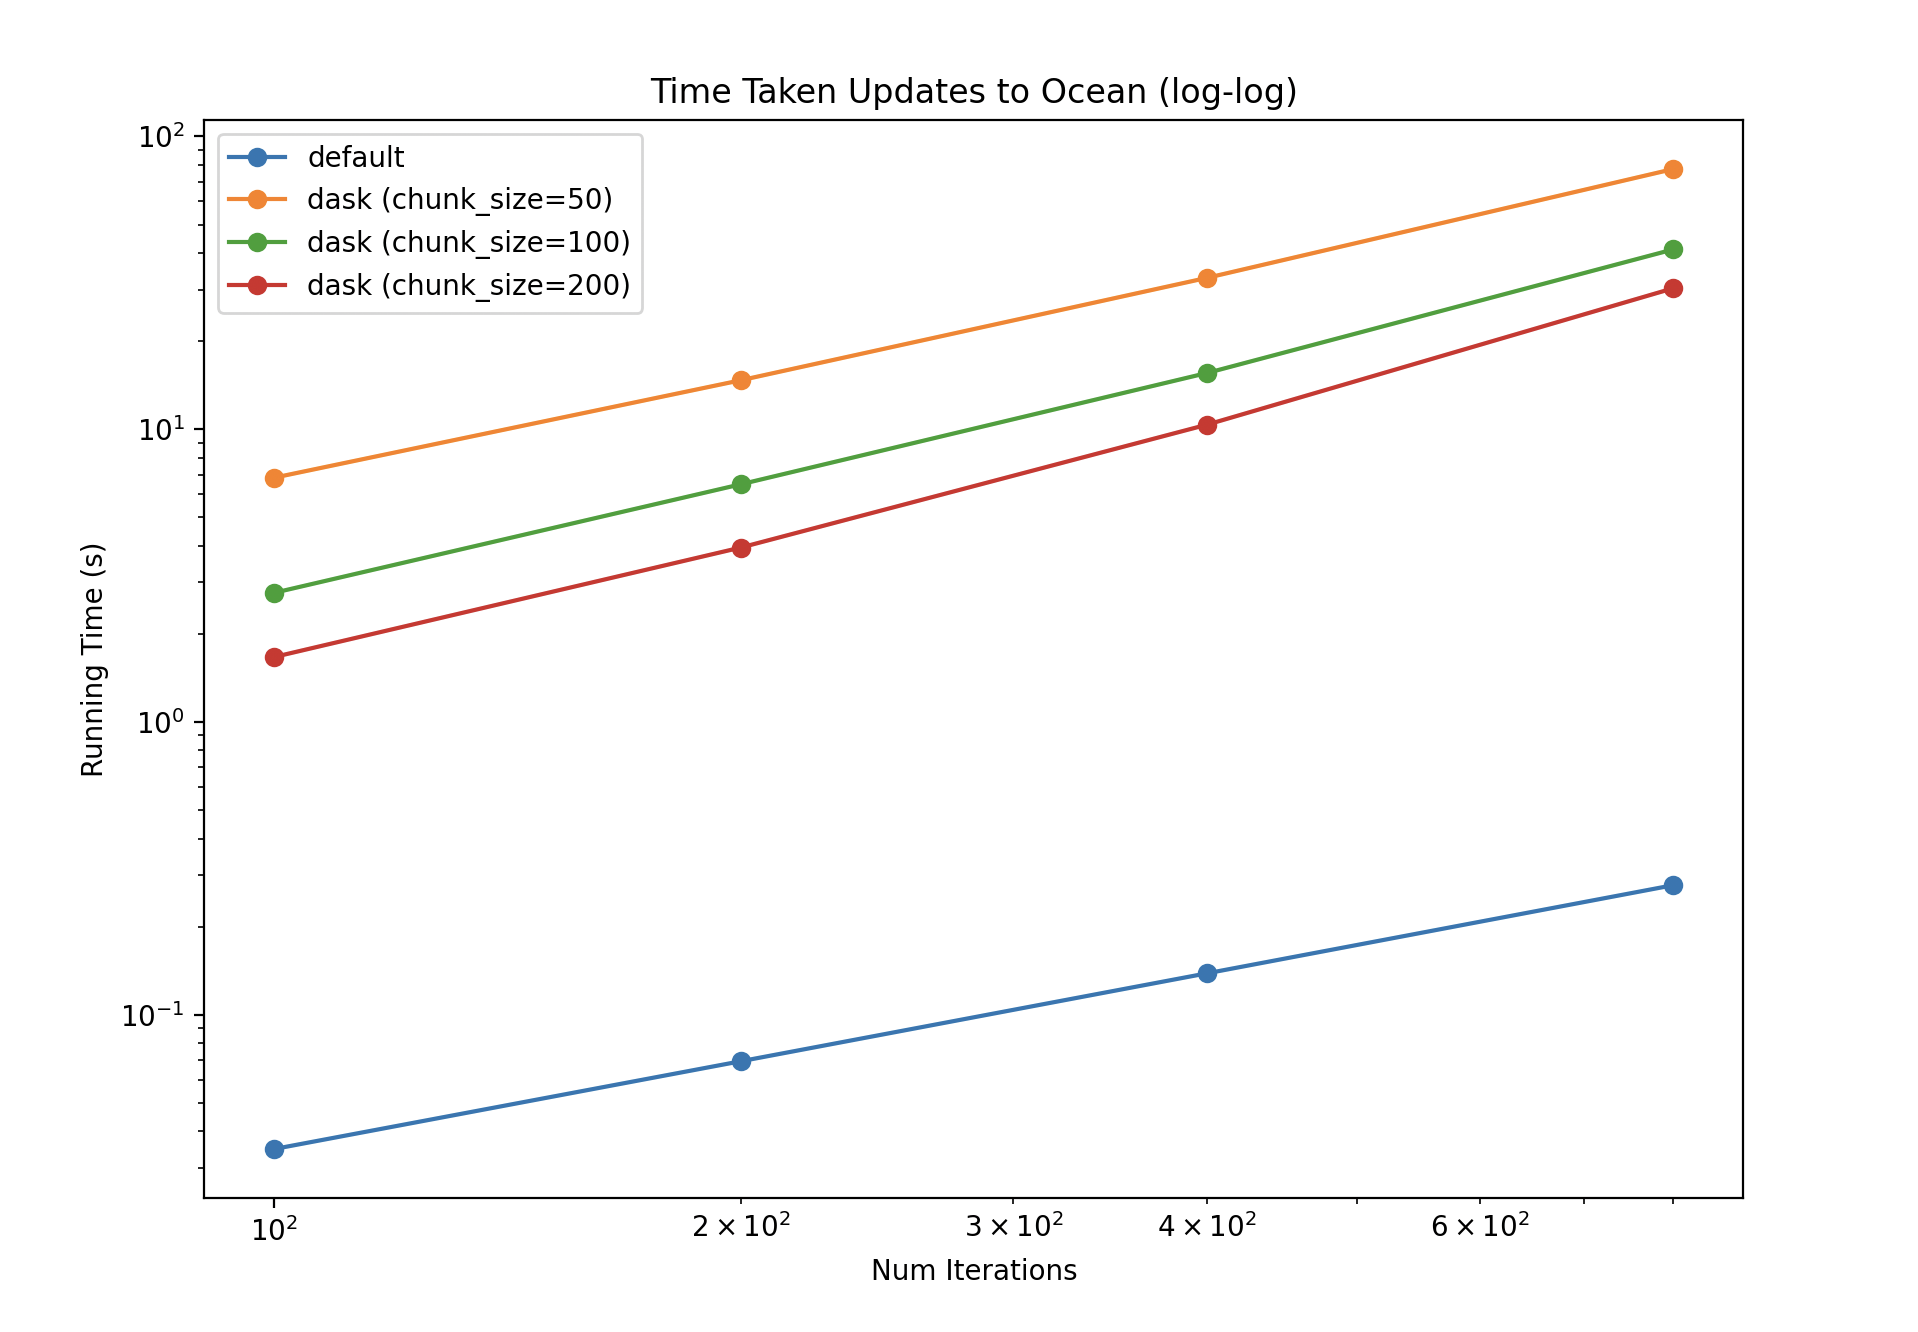
\includegraphics[width=0.8\textwidth]{../images/bonus_default_dask_runtimes.png}
  \caption{Running Time Comparisons For Dask and Default Ocean Updates}
\end{figure}

The first thing that stands out is that the \textbf{default (numpy) implementation outperforms Dask} implementations for all three chunk sizes.
We believe that this can largely be attributed to the fact that Dask parallelization with the help of \verb|map_overlap| has the overhead of chunk creation, ghost cell management, appropriate wrapping around boundaries (for the \verb|periodic| boundary type), etc.
On top of this, Dask needs to manage -- among other things -- the intermediate task graphs or the scheduling of workloads.
Additionally, Dask also seems to assume that the underlying memory infrastructure is not one that uses shared-memory, and thus communicates between the different chunks that are created (as explained \href{https://canvas.kth.se/courses/52247/discussion_topics/452810}{here}). 

\verb|numpy| does not add any of the above complexity.
It appears that there are \textbf{\underline{no advantages in terms of runtime}} of parallelizing this computation using Dask and \verb|map_overlap| on a \underline{shared-memory architecture}, such as the 2021 M1 laptop. 

Second to note is that for \textbf{smaller chunk sizes, runtime increases}.
This agrees with our expectations.
Smaller chunk sizes mean more chunks, which in turn would lead to more communication between those.
This then adds to the overhead of using Dask and increases the runtime.
In practice we denote $50 \times 50$ chunks performing the worst, and $200 \times 200$ chunks performing the best when using Dask.

For completeness, we would close by noting that the runtime increases across all implementations as the number of iterations increases, as is expected.

\subsection{Performance Monitoring using Dask Dashboard}
For performance monitoring, we utilized the Dask Dashboard made available on using the \verb|dask.distributed| module's \verb|Client| class.
We let Dask decide the default number of workers and threads per worker for the 2021 M1 MacBook Pro (16 inch) machine -- which was \textbf{5 workers, each with 2 threads}.
The performance monitpring code can be found in the \verb|main| function of the \verb|ocean_dask.py| file.

\subsubsection{Task Stream \& Worker Monitoring}
We observed the \textbf{Task Stream} panel and the \textbf{Workers} panel of the Dashboard for the Dask-parallelized runs of the ocean simulation for 100 iterations.
We used a chunk size of $100 \times 100$ -- resulting in \underline{4 chunks} being created for the origial $200 \times 200$ grid.
\textit{Note: The chunk-size will be varied in the next section. For this section, we only talk about chunk-size of $100 \times 100$}. 
On doing so, we observed the following on the \textbf{Task Stream} panel:

\begin{figure}[H]
  \centering
  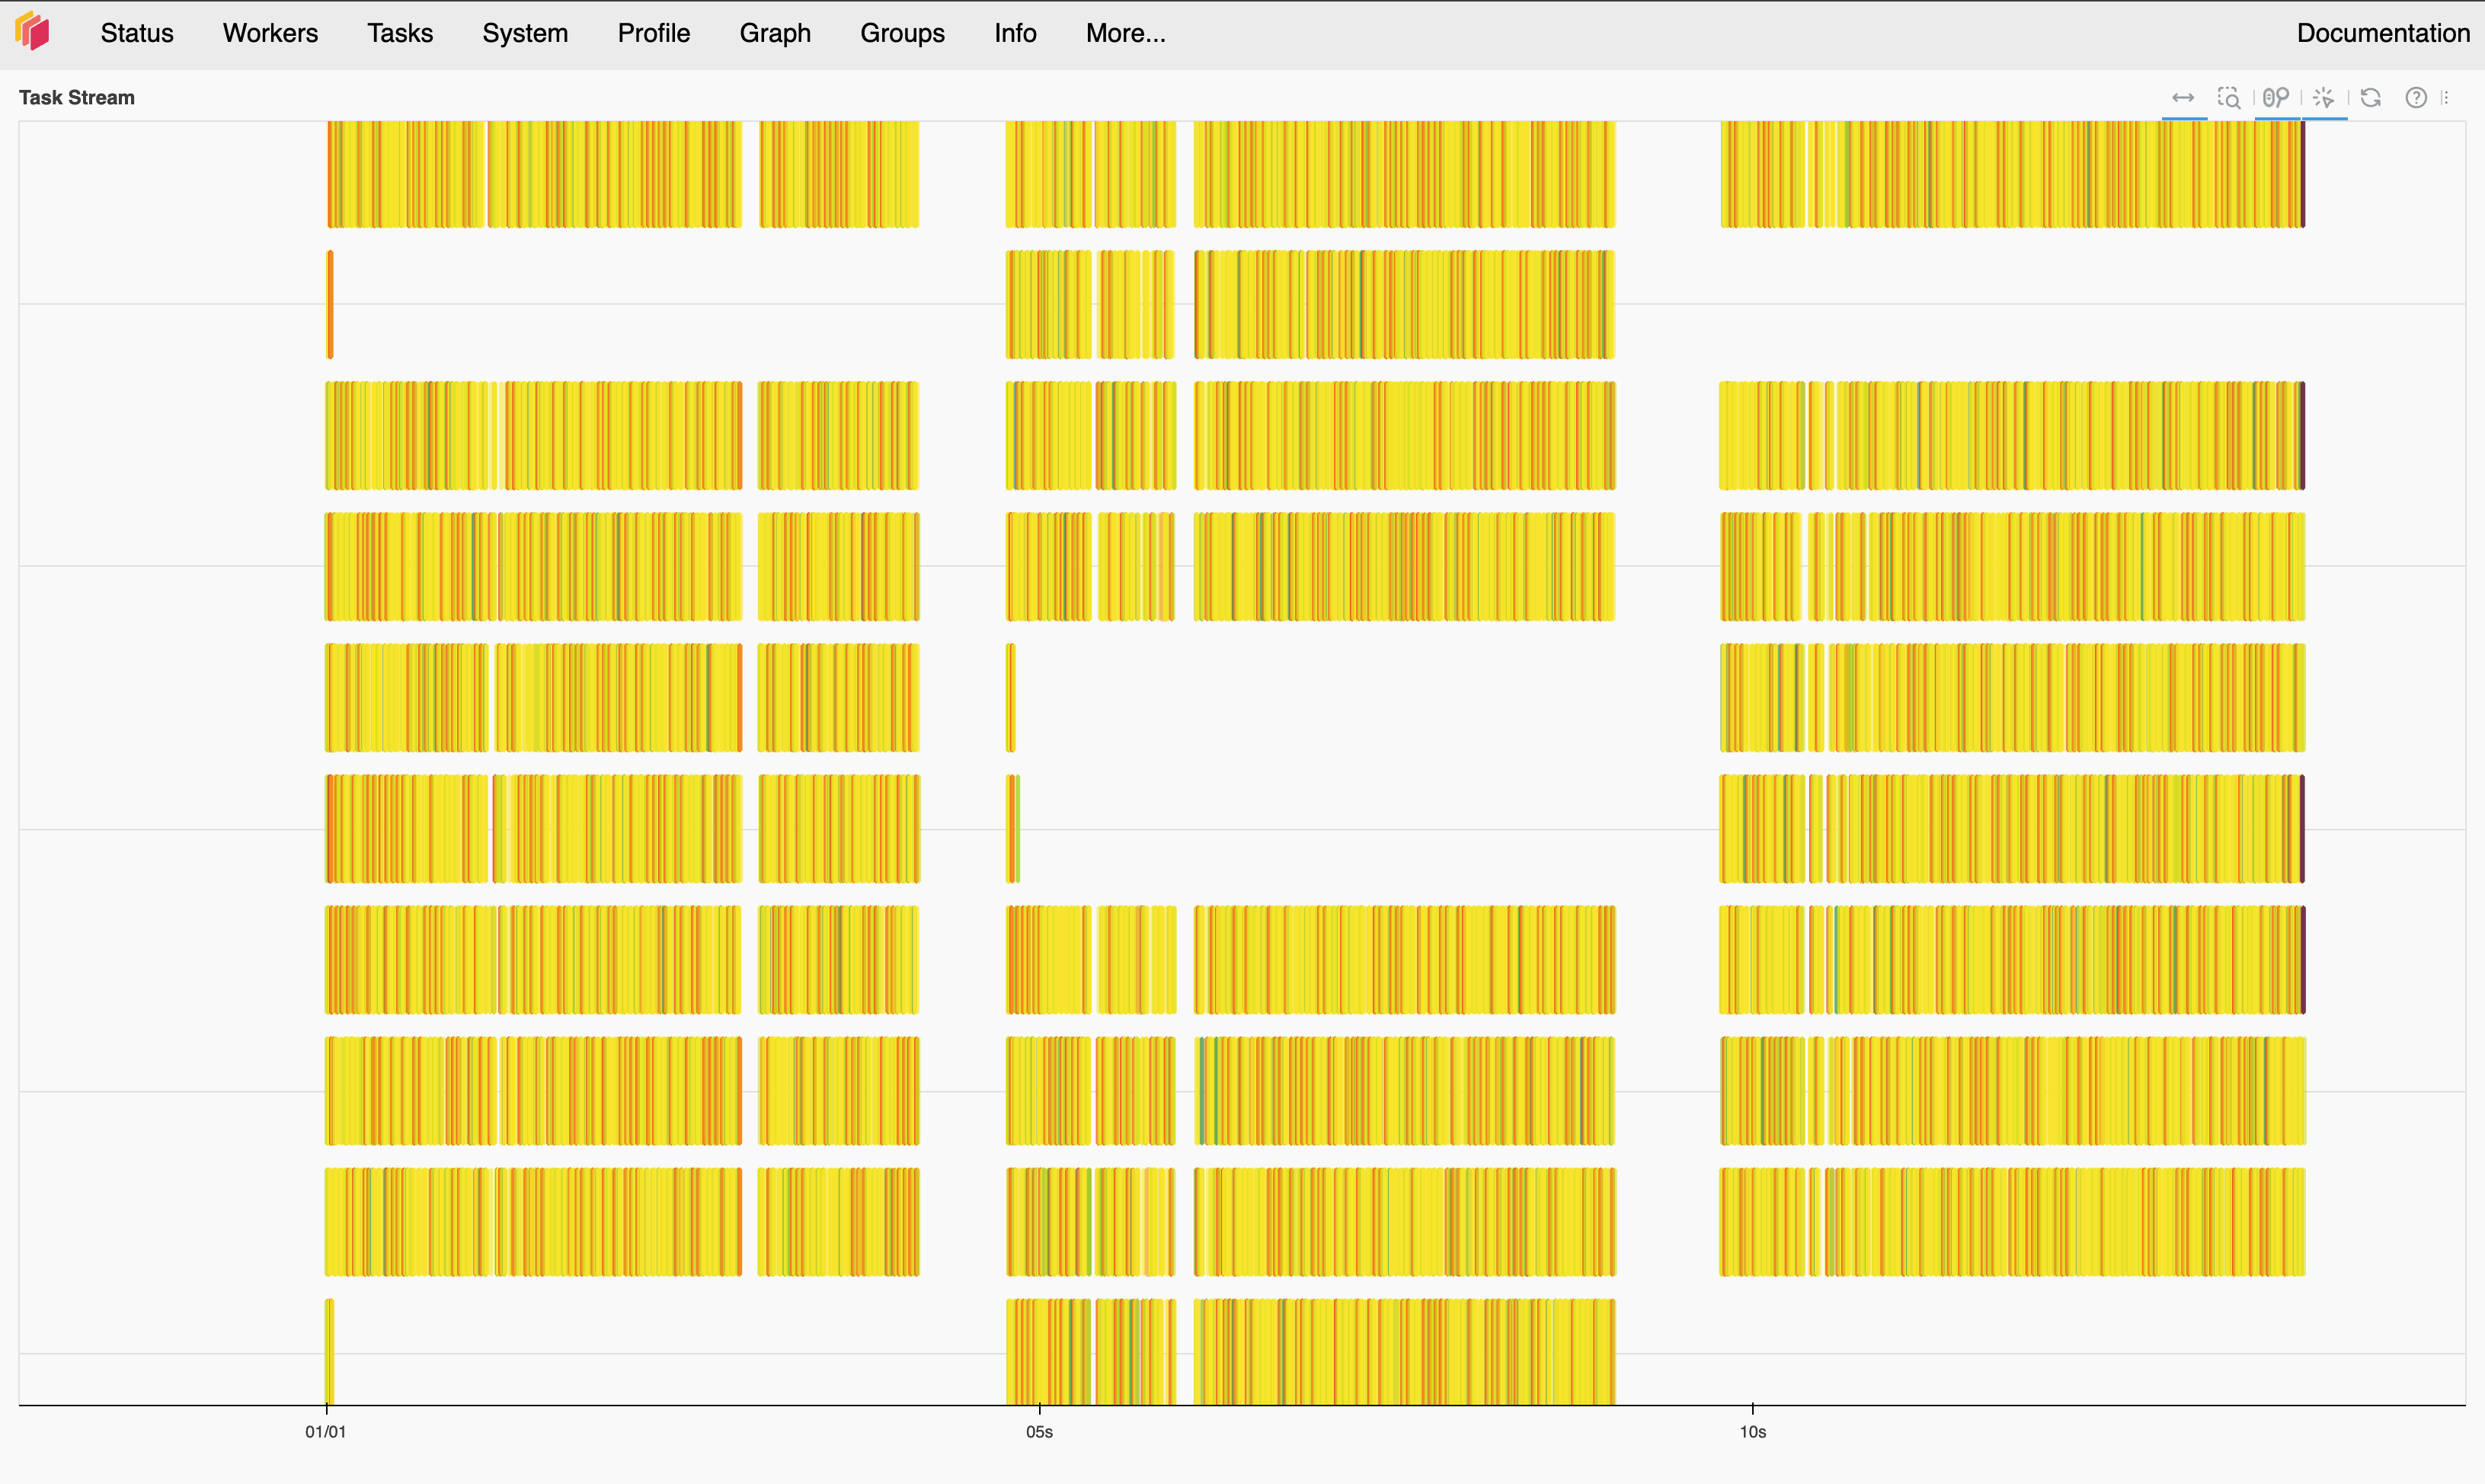
\includegraphics[width=0.8\textwidth]{../images/task_stream_100chunk.png}
  \caption{Task Stream For Ocean Simulation Using Chunk Size $100 \times 100$}
\end{figure}

To help interprete this result, we referred to the official Dask documentation: \url{https://docs.dask.org/en/latest/dashboard.html#task-stream}.
It is immediately evident that we observed a notable count of \textbf{red rectangles}, indicating that there is a non-trivial amount of communication between workers.
This relates to the disappointing runtime results on a shared-memory architecture discussed above.

Next we observed that there were 3 \textit{bursts} of computation.
All workers seem to have no activity for a short \textit{rest} period between these 3 bursts.
The Dask Documentation states that each row \underline{corresponds to a thread} that was involved in the computation at some time.
In each burst, there were \textbf{2 threads} with minimal participation in the computation.
Since each worker has 2 threads in our setup, it leads us to believe that there was 1 worker in each \textit{computation burst} that had minimal to no contribution.
There are only four chunks to distribute amongst workers (for a $100 \times 100$ chunk size), ergo there has to be one worker among five who would not be participating in the computation. 

We also observe this in the \textbf{Workers} tab of the Dask Dashboard
For a chunk size $100 \times 100$ we can see the evolution of the CPU Usage of the five workers.
A video recording is available at \href{https://github.com/paulmyr/DD2358-HPC25/tree/master/04_parallel/bonus#chunk-size-100}{link}.
Here we can note that Worker 3 has minimal participation (as observed from the CPU Usage) for the first \textit{burst} of computation, followed by Worker 4 in the second \textit{burst}, and finally by Worker 1 in the final \textit{burst}.
The CPU Usage from each worker usually does not exceed the \textbf{35-40\%} range
It indicates that the workers are not being overburdned by computation.
Similarly, the Memory Usage of each worker is well below the limit throughout the course of the computation (never getting close to the 3.2 GiB limit per worker).

This brings us to the conclusion, that the runtime is neither limited by memory nor CPU usage.
It is rather the overhead involved in communicating between workers and the background tasks involved with scheduling workloads, ghost-cell overlaps, etc.
The generalization techniques Dask uses cannot show their potential on a shared-memory architecture.

\subsubsection{Experiment with Different Chunk Sizes}
\label{sec:experiment_with_different_chunk_sizes}
We varied the \textbf{chunk sizes} to see how this would impact the task distribution and workload on the five workers.
First, we will talk about what we observed on \textbf{Task Stream} panel (for workload distribution, communication between workers, etc), followed by our observations of the \textbf{Workers} panel (for CPU and Memory Usage per worker). For this, we kept the same number of iterations (100) as in the previous section.

\begin{itemize}
\item \textbf{\underline{$50 \times 50$ Chunk Size}} \\
  With a chunk-size of $50 \times 50$, we had in total 16 chunks for the $200 \times 200$ grid(s).
  Since we increased the number of chunks involved in the computation, we expected an increase in the number of communication between workers (or, inter-worker communication) -- this would in-turn lead to a slowdown in the computation being performed.
  In the \textbf{Task Stream} panel we observe an \textbf{increased number of red rectangles}, denoting an higher inter-worker communication.
  This also \textit{increases scheduling overhead} -- which is what the handout was referring to.

\begin{figure}[H]
  \centering
  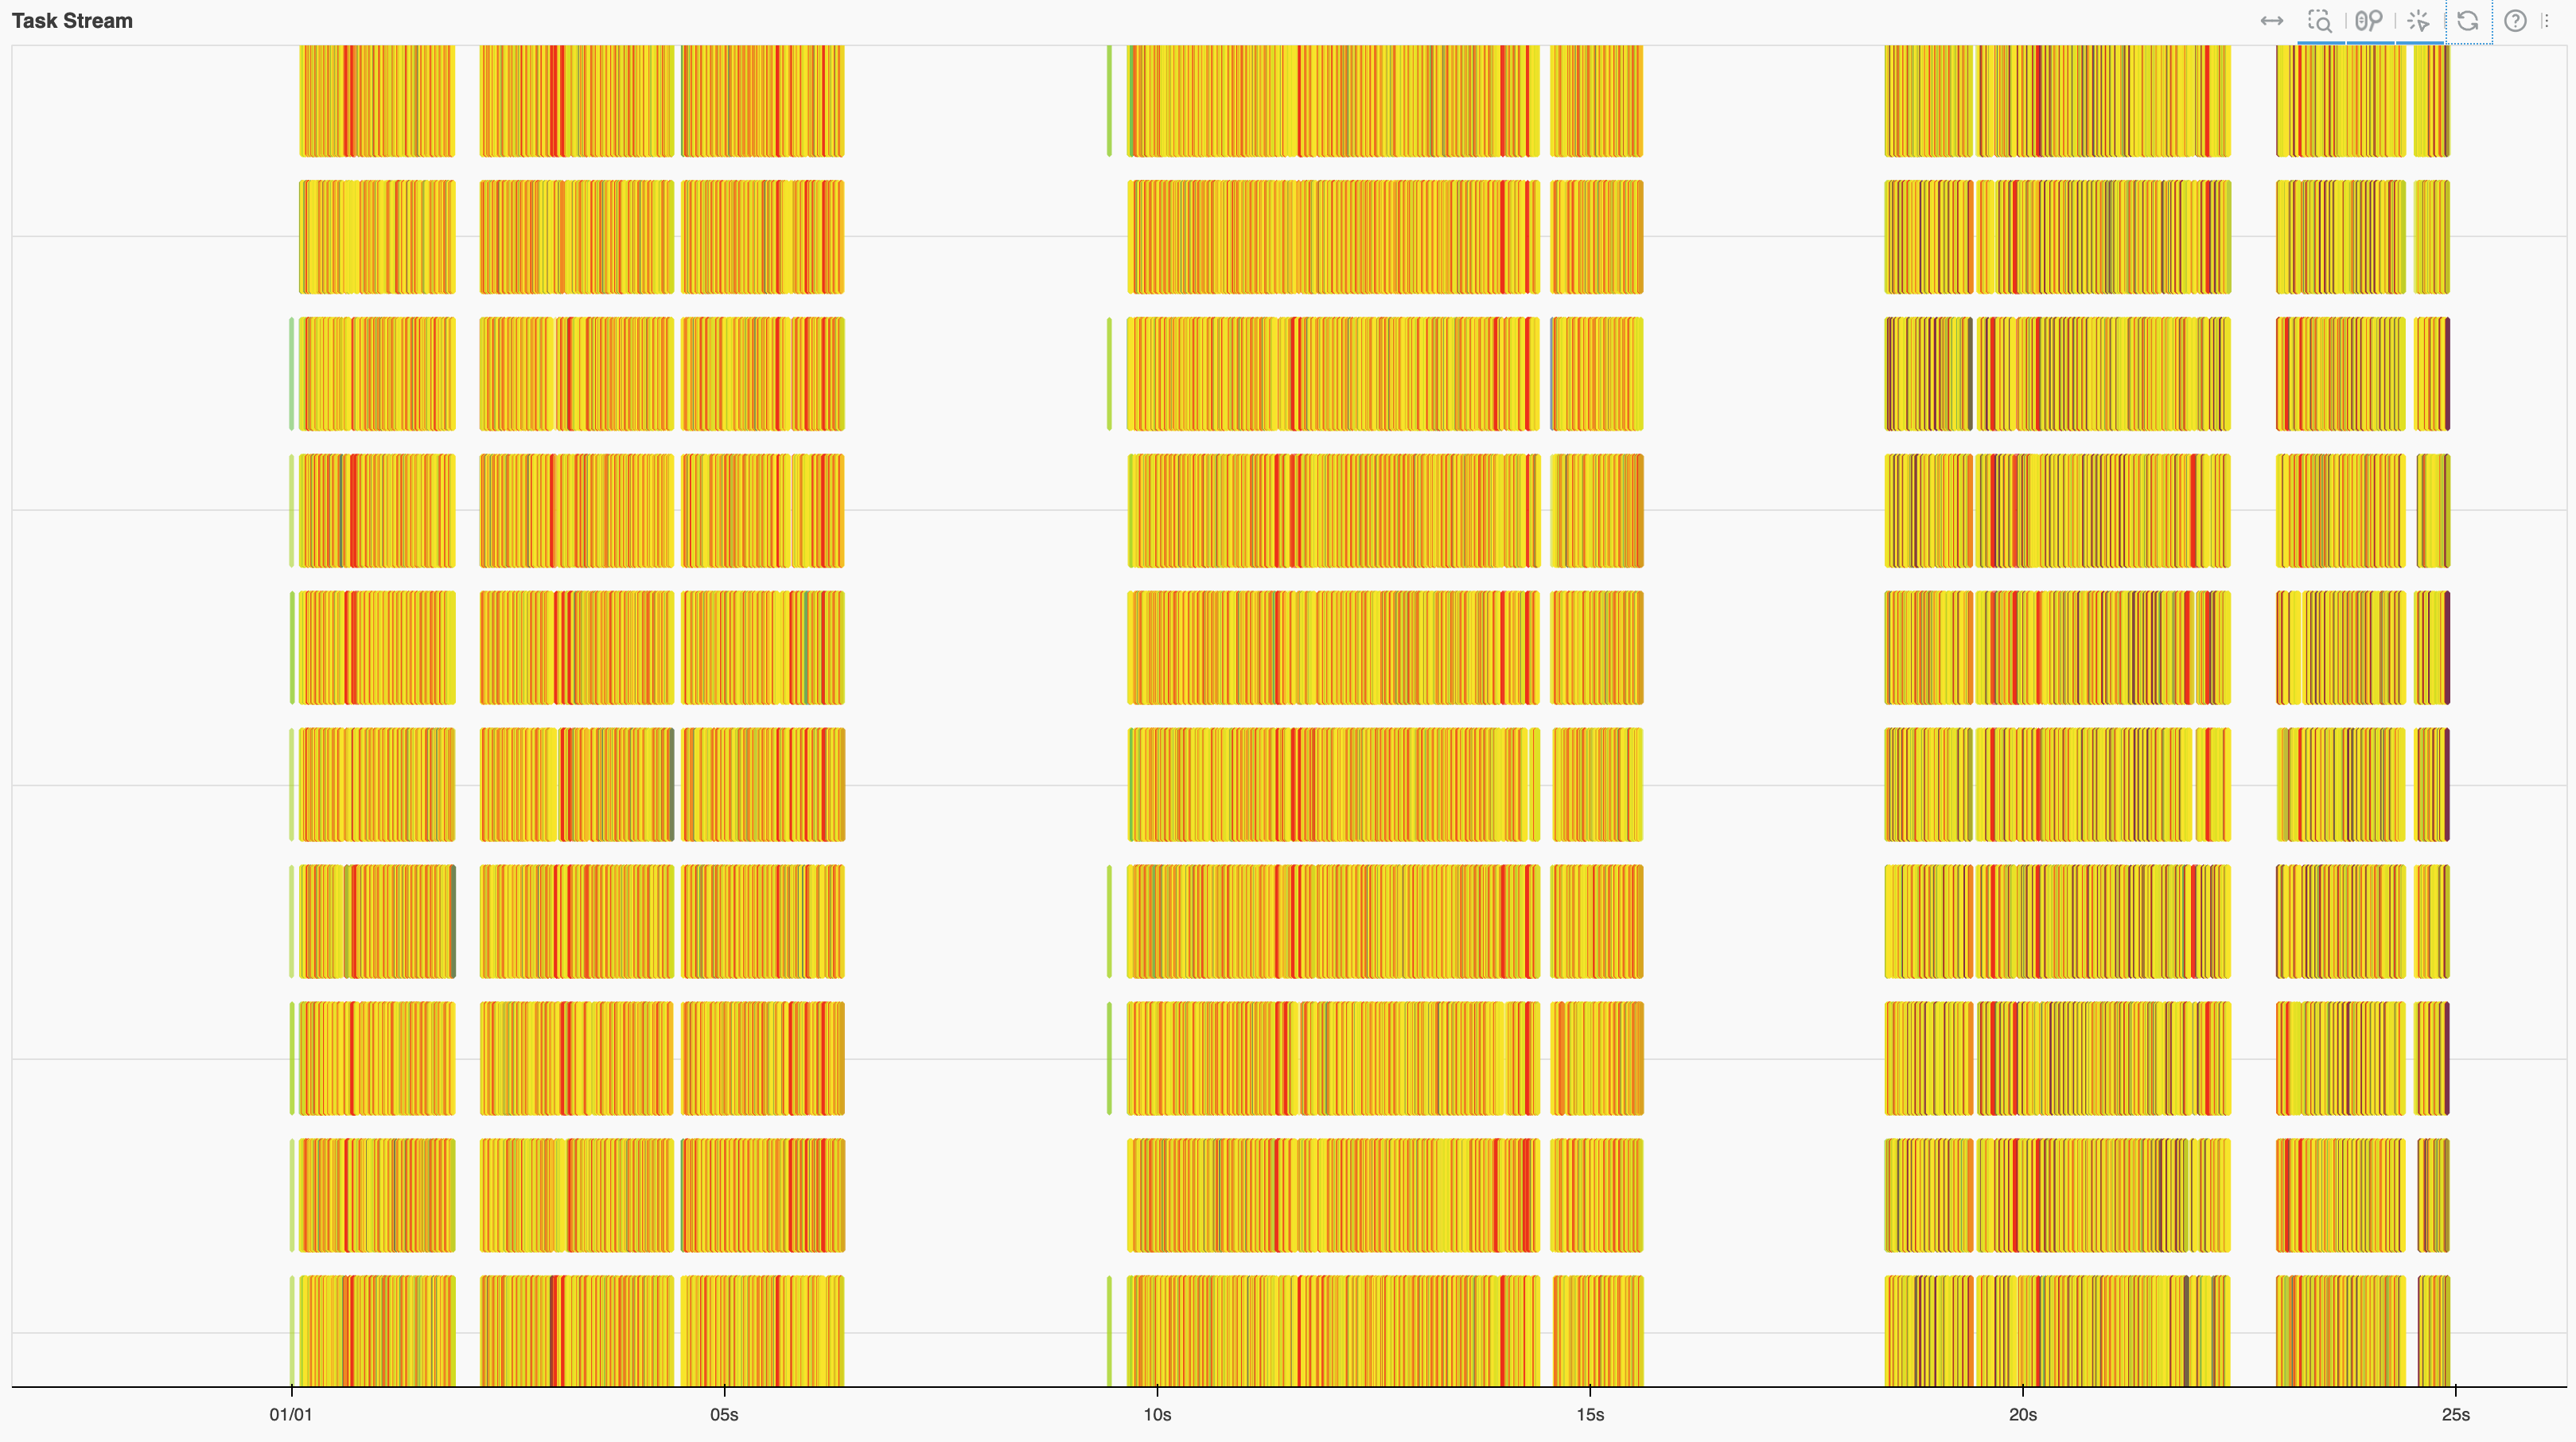
\includegraphics[width=0.8\textwidth]{../images/task_stream_50chunk.png}
  \caption{Task Stream For Ocean Simulation Using Chunk Size $50 \times 50$}
\end{figure}

We also observe that while there were similar \textit{bursts} of computation across workers that we saw in the \textbf{Task Stream} for $100 \times 100$ chunk size above, in all these bursts, \textbf{all threads/workers had some contribution to the computation}.
This makes sense -- now we have more chunks than workers.
Each worker (and thus thread) is always involved in the computation.
No single worker is overburdned, even though the computation is suboptimal because of the scheduling overhead.

This pattern can also be recoginzed on the \textbf{Workers} panel, where during each \textit{computation burst}, all workers are involved in the computation.
A video demonstration showing the evolution of the Worker statistics over the course of a computation using $50 \times 50$ chunk sizes can be found here: \href{https://github.com/paulmyr/DD2358-HPC25/tree/master/04_parallel/bonus#chunk-size-50}{link}.
In fact, the CPU Usage per worker seems to be \textbf{higher} than what was observed in the $100 \times 100$ chunk-sizes case of the previous section.
We feel that this could potentially be attributed to a higher number of inter-worker communication, which should be a result of a higher number of chunks over which the computation is being performed. 

However, there is \textbf{no noticable difference in memory consumption} in the $50 \times 50$ chunk size case compared to the $100 \times 100$ case.
Dask therefore does not increase the memory overhead notably by increasing the number of chunks.

\item \textbf{\underline{$100 \times 100$ Chunk Size}} \\
We had a discussion about the Task Stream and Workers panel in the $100 \times 100$ chunk-size case in the previous section, so we refrain from repeating that here. Please refer to the previous section for our analysis.

\item \textbf{\underline{$200 \times 200$ Chunk Size}} \\
  When working with a chunk-size of $200 \times 200$, there is only one chunk to work with, and 5 workers (10 threads).
  We expected inter-worker communication to be \textbf{minimal} and resulting in \textbf{(very) few red rectangles} in the Task Stream graph; which is exactly what we observed.
  This contributes to the fact that a chunk size of $200 \times 200$ being the quickest simulation amongst the different chunk-size configurations we tried.

\begin{figure}[H]
  \centering
  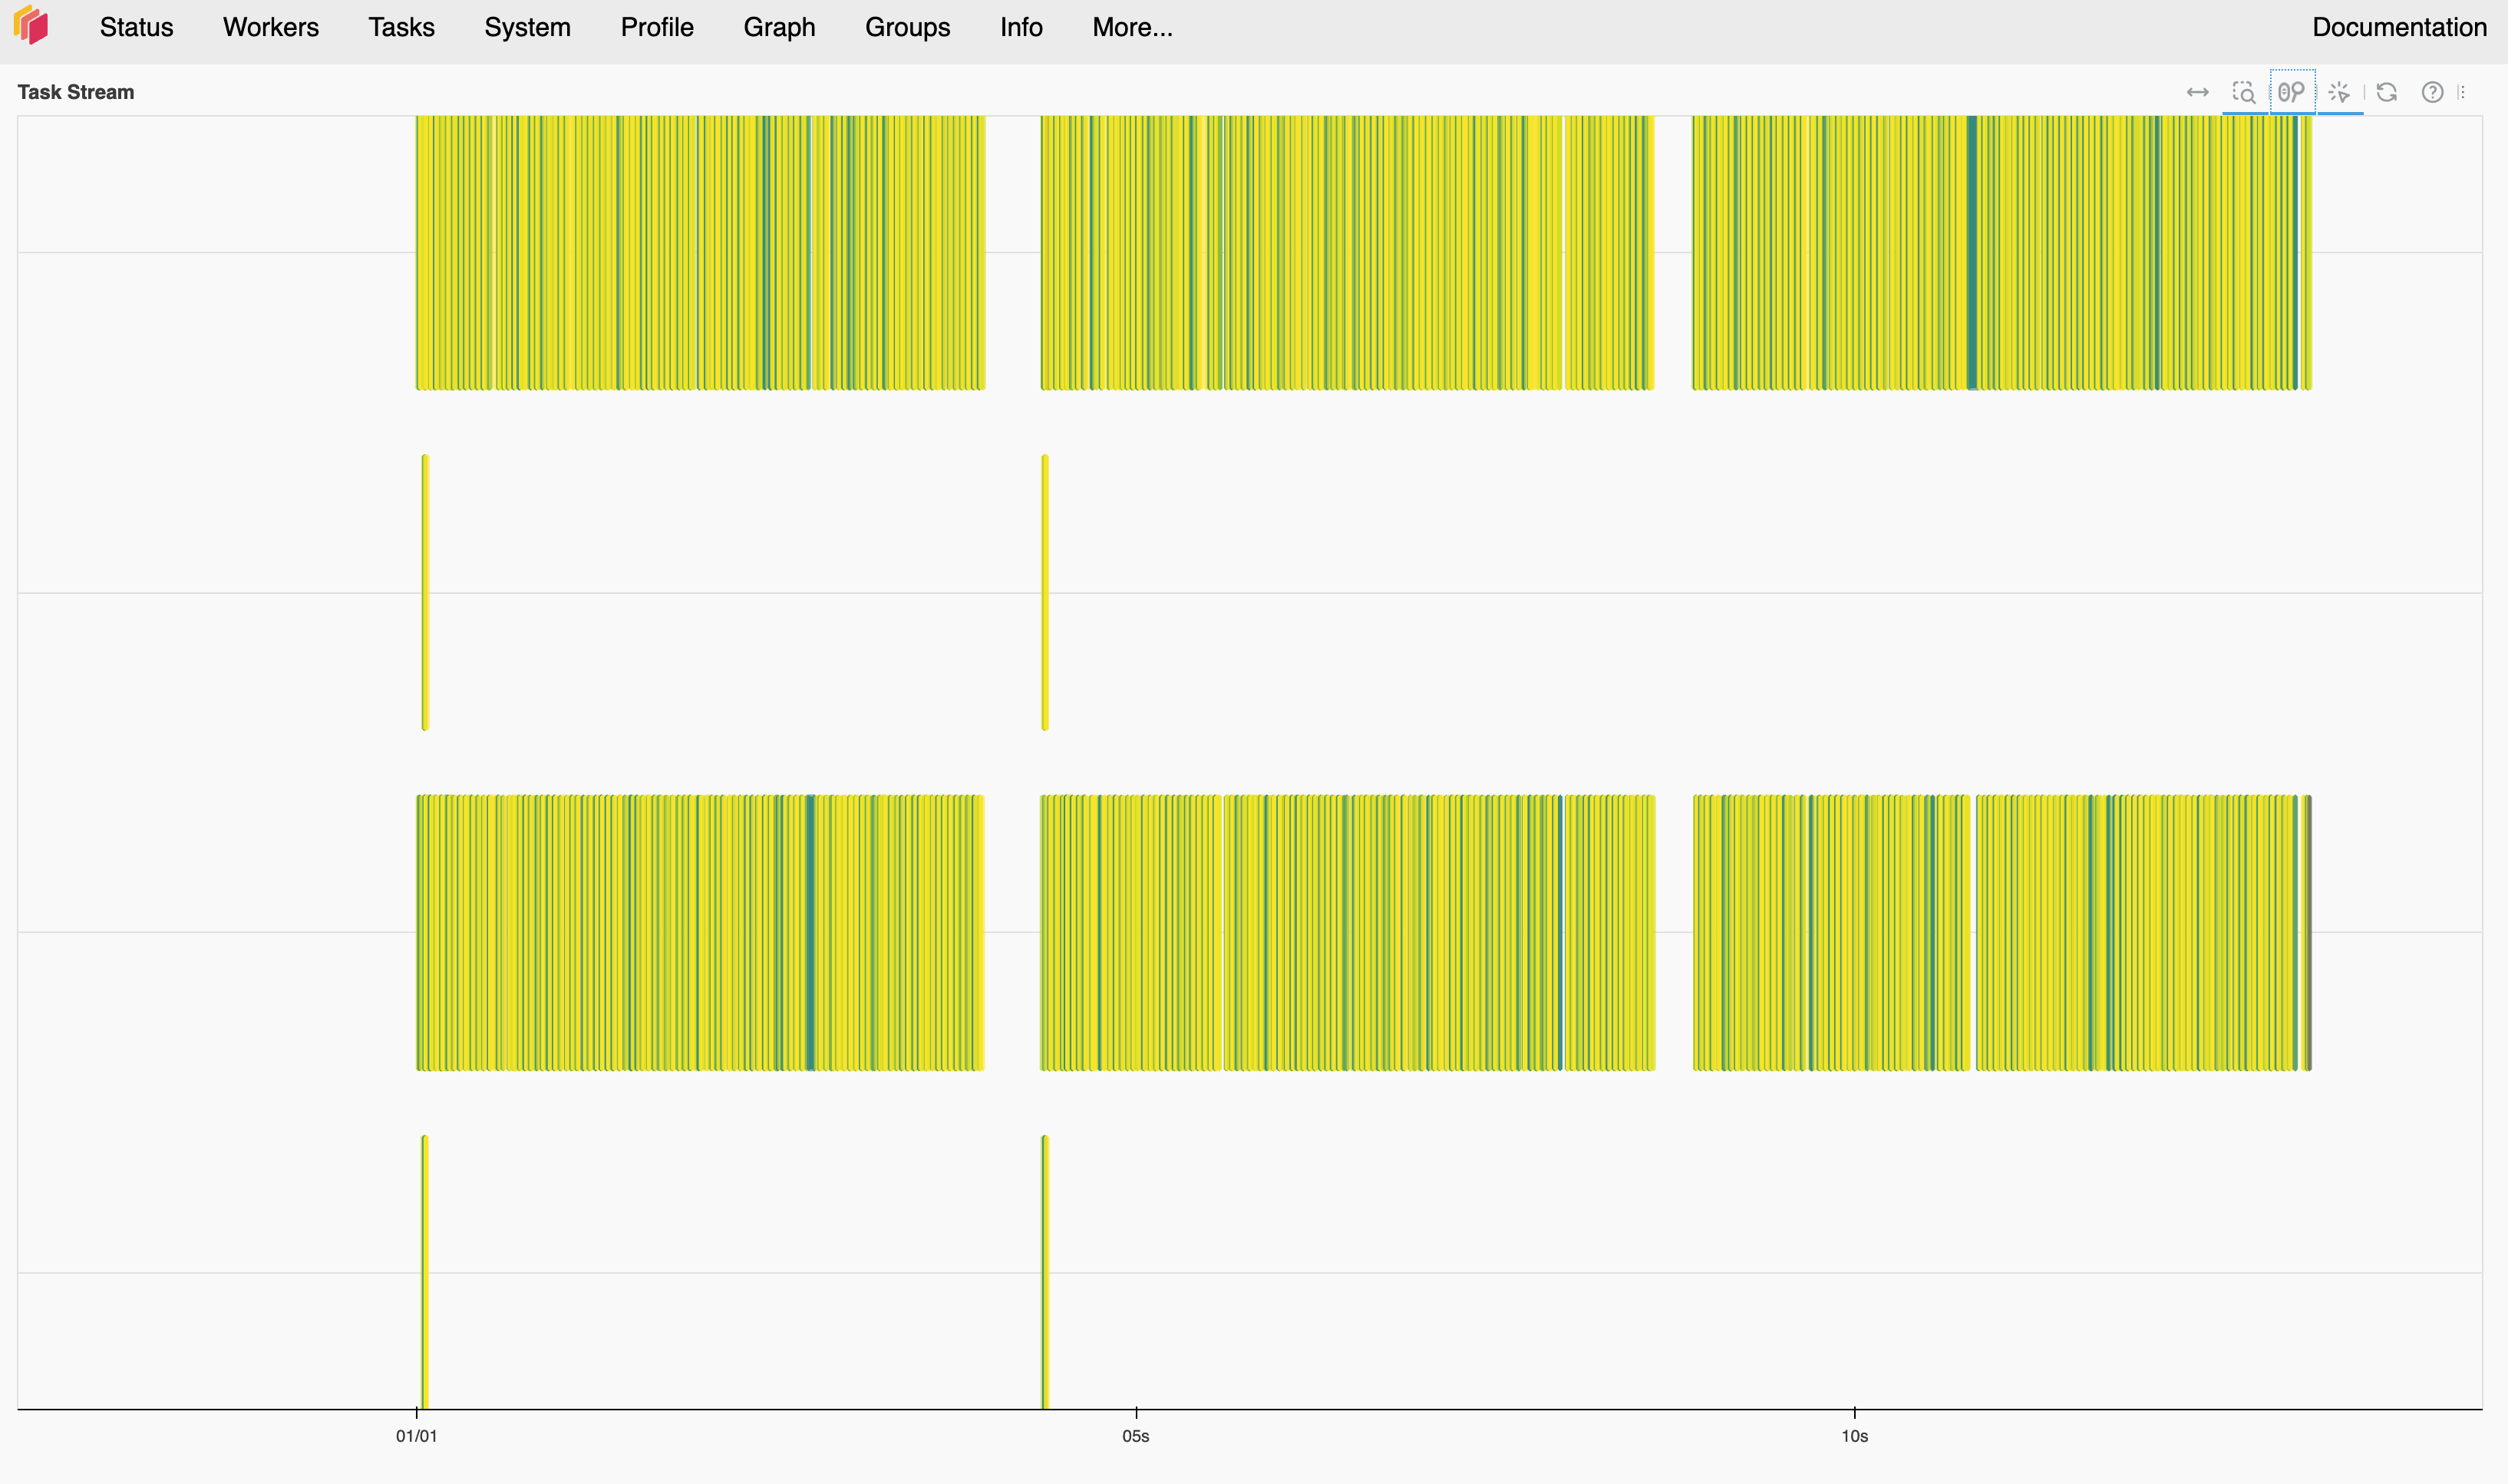
\includegraphics[width=0.8\textwidth]{../images/task_stream_200chunk.png}
  \caption{Task Stream For Ocean Simulation Using Chunk Size $200 \times 200$}
\end{figure}

Of note here is that we only see four threads (or 2 workers) in the Task Stream visualization for a computation with $200 \times 200$ chunk size. Based on the Dask Documentation, we believe this indicates that Dask only uses these four threads (out of 10) to perform this computation.
This behaviour is to be expected.
Due to only one chunk beeing distributed amongst five workers, the heavy computational work cannot be done in parallel.
While two workers are working on the computation (see \href{https://github.com/paulmyr/DD2358-HPC25/tree/master/04_parallel/bonus#chunk-size-200}{link}) only one worker has any significant cpu load.
We assume the other worker is tasked with overhead duty.
Still, this performs best out of the three scenarios we tested.
This again indicates that this form of parallelization on a shared-memory architecture is suboptimal.

A similar story is being told in the evaluation of the information provided within the \textbf{Workers} panel.
For a computation with a chunk-size of $200 \times 200$ you may find a recording of the output here: \href{https://github.com/paulmyr/DD2358-HPC25/tree/master/04_parallel/bonus#chunk-size-200}{link}.
As can be seen in the video, once the computation starts, workers 0 - 2 and 4 are idle.
Worker 3 performs the computation, which is evident from its CPU Usage percentage over the course of the computation.

\item \textbf{\underline{Conclusion}}\\
  In conclusion, on varying the chunk sizes while keeping the number of iterations and workers the same in the aforementioned setup, we observe that a \textbf{decrease in chunk size} leads to an \textbf{increase in inter-worker communication}
  We determine this to be the main factor in the increase of runtime compared to a shared-memory optimized implementation.

  Increasing the chunk-size decreases the number of chunks available.
  In turn this results in some workers being idle.
  This is no short-coming of the Dask Scheduler -- it seems to perform reasonably well at ensuring all workers having similar work loads, given \underline{enough chunks are available}.
  Also, Dask seems to prefer picking the same worker across different \textit{bursts} of computation.
  This may be reletated to enforcing cache coherency.
  We also \textbf{did not observe} any noticable differences in \textbf{memory load or consumption} when varying chunk-sizes.
  Each worker seemed to use somewhat the same amount of memory, no matter the chunk size.
  We may contribute this to the fact, that the acutal memory needed for the computation is actually outweighed by the Dask worker memory overhead.
  Because the size of the entire grid being comparatively small (at a constant $200 \times 200$), we would need to greatly increase the grid size to make sure each worker does not run out of memory.

  To put it in a nutshell, we believe that this profiling illustrates how \textbf{managing chunks amongst different workers} is potentially a \textbf{significant contributor to increased runtime} when using Dask-Array parallelization as opposed to the serial numpy implementation on shared-memory architectures.
  It outweighs the benefits of parallelization and appears to be \textbf{suboptimal in regards to improving performance} given our setup.
  Our conclusion might change revisiting this implementation on a distributed architecture. 
\end{itemize}

\subsubsection{Miscellenaeous Questions}
Based on our observations and thorough discussion above, we now answer some miscellaneous questions presented to us at the end of the \textit{Bonus} section.

\begin{itemize}
\item \textbf{\underline{How well-balanced were the worker loads?}}\\
  It depends on the chunk size: small chunk sizes improved balancing at the cost of communication and vice versa.

  To us, this seems logical, and we do not think that the Dask Scheduler is to be blamed for this. As a minor improvement/alternative, however, one could say that the Dask Scheduler could attempt to "distribute" the smaller number of chunks more democratically across workers. For example, in the $200 \times 200$ case, we saw that only one worker \textbf{throughout the computation} did a bulk of the job.
  We attributed this fact for exploiting cache coherence.
  One alternative of this could be to try and have other workers involved as well -- for instance, Worker 0 could do the computation during the first \textit{burst}, Worker 2 could take-over in the second \textit{burst}, etc.
  One downside of this is that if there are dependencies in the computation between bursts, then this could lead to more memory I/O between workers in a more general setting, which might explain why Dask prefers to keep computation on a single worker in the $200 \times 200$ scenario.
  Also the computation might be run on a different CPU core, which would lead to storing and restoring all cache values from the registers.
  Thus, overall, we feel that this might decrease performance in the case of low number of chunks.
  The current Dask scheduling seems to be doing a democratic job for higher number of chunks.

\item \textbf{\underline{Did any worker run out of memory?}}\\
  Based on our observations of the Worker panel across different chunk-sizes, \textbf{no worker} seems to run out of memory.

\item \textbf{\underline{Was there idle time or task queueing?}}\\
  For all chunk-sizes, we did notice idle time between the \textit{computation bursts} that we were referring to earlier.
  We believe that this idle time could be attributed to the threads/workers waiting for the scheduler to allocate and distribute new jobs to them.
  This "pause" between \textit{computation bursts} increases with an increase in the \textbf{number of chunks}, which indicates that it might be due to additional load on the scheduler.

  Idle times also appear when fewer chunks than workers are available (see discussion \ref{sec:experiment_with_different_chunk_sizes}

  Finally, to examine if there was any task-queuing, we looked at the \textbf{Progress} panel (available from under \textbf{More...}) on the Dask Dashboard.
  For all 3 chunk sizes, we observed that there was \textbf{no task queuing}, as can be seen for the video demonstration over the course of the computation for each chunk-size in the code repository (see: \href{https://github.com/paulmyr/DD2358-HPC25/tree/master/04_parallel/bonus#chunk-size-50-1}{$50 \times 50$}, \href{https://github.com/paulmyr/DD2358-HPC25/tree/master/04_parallel/bonus#chunk-size-100-1}{$100 \times 100$}, \href{https://github.com/paulmyr/DD2358-HPC25/tree/master/04_parallel/bonus#chunk-size-200-1}{$200 \times 200$}).
  For each of these videos, we looked at the \verb|queued| number at the top of the panel, which remains 0 throughout the computation.
  We expect this to mean that there were \textbf{no queued tasks} for all chunk-sizes over the course of the computation.

  Based on the Dask Documentation (\href{https://distributed.dask.org/en/stable/scheduling-state.html#task-state}{link}), a queued task is "Ready to be computed, but all workers are already full".
  It means that all the dependencies required for computing the task are ready, but no worker is available to perform the computation.
  There were no tasks with this status throughout.
  However, there were tasks with the status \verb|waiting|, which according to the documentation means that the task is "On track to be computed, waiting on dependencies to arrive in memory".
  We conclude that for our computation, once the dependenceis required to compute the task arrived in memory, the task was assigned almost immediately to a worker (or assigned quick enough for it not to receive a \verb|queued| status) by the scheduler.
\end{itemize}

\subsubsection{VTK Files and Paraview}
The serial implementation allows for easy saving of the computed data, ergo the ocean temperature and current velocity to vtk files every few time-steps.
For visualization purposes, the total \verb|TIME_STEPS| was increased from 100 to 1000.
As with Exercise 1, only the serial implementation's data was saved to VTK files, which are present under the \verb|vtk/| subdirectory of the \verb|bonus/| directory for this assignment.

The entire animation for both the temperature (\href{https://github.com/paulmyr/DD2358-HPC25/blob/master/04_parallel/bonus/README.md#temperature-visualization}{link}) and the velocity (\href{https://github.com/paulmyr/DD2358-HPC25/blob/master/04_parallel/bonus/README.md#velocity-visualization}{link}) can be found in the \verb|README.md| for the \verb|bonus/| subdirectory of this assignment.
Here, we provide 5 screenshots for both visualizations, taken every 250 loop iterations.

 \begin{figure}
\centering
\begin{subfigure}{0.4\textwidth}
    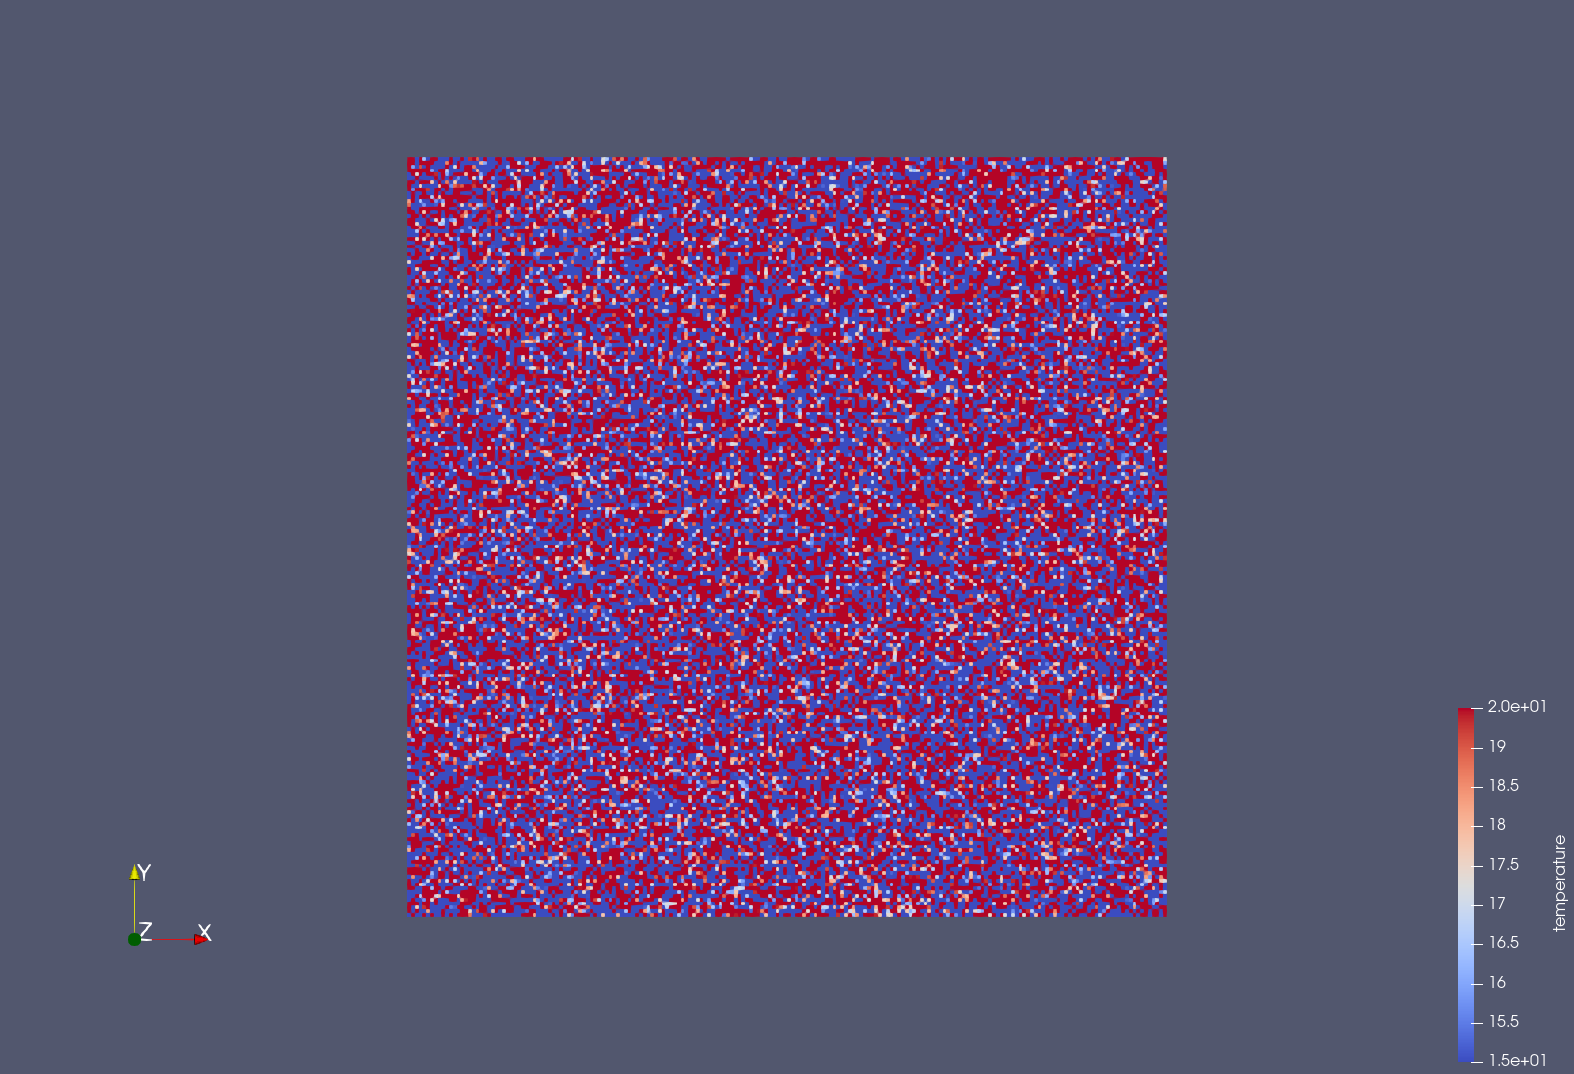
\includegraphics[width=\textwidth]{../images/vtk/bonus/temp/step_0.png}
    \caption{Time step 0}
\end{subfigure}
\hfill
\begin{subfigure}{0.4\textwidth}
    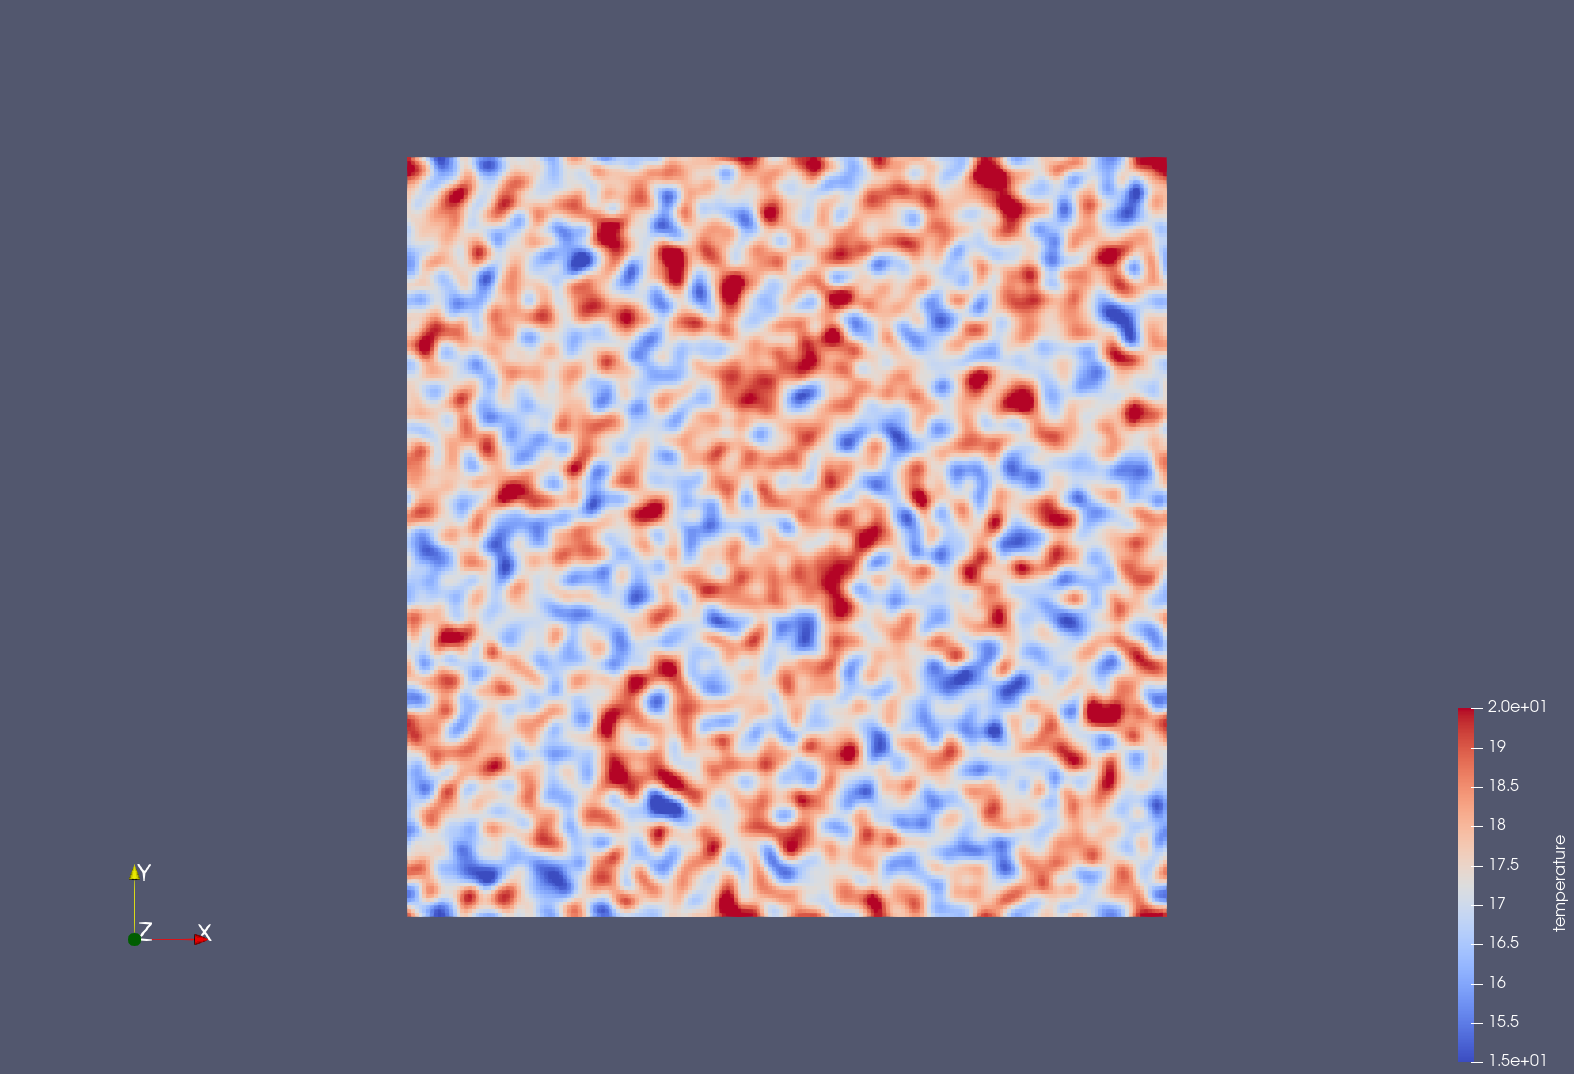
\includegraphics[width=\textwidth]{../images/vtk/bonus/temp/step_25.png}
    \caption{Time step 250}
\end{subfigure}
\hfill
\begin{subfigure}{0.4\textwidth}
    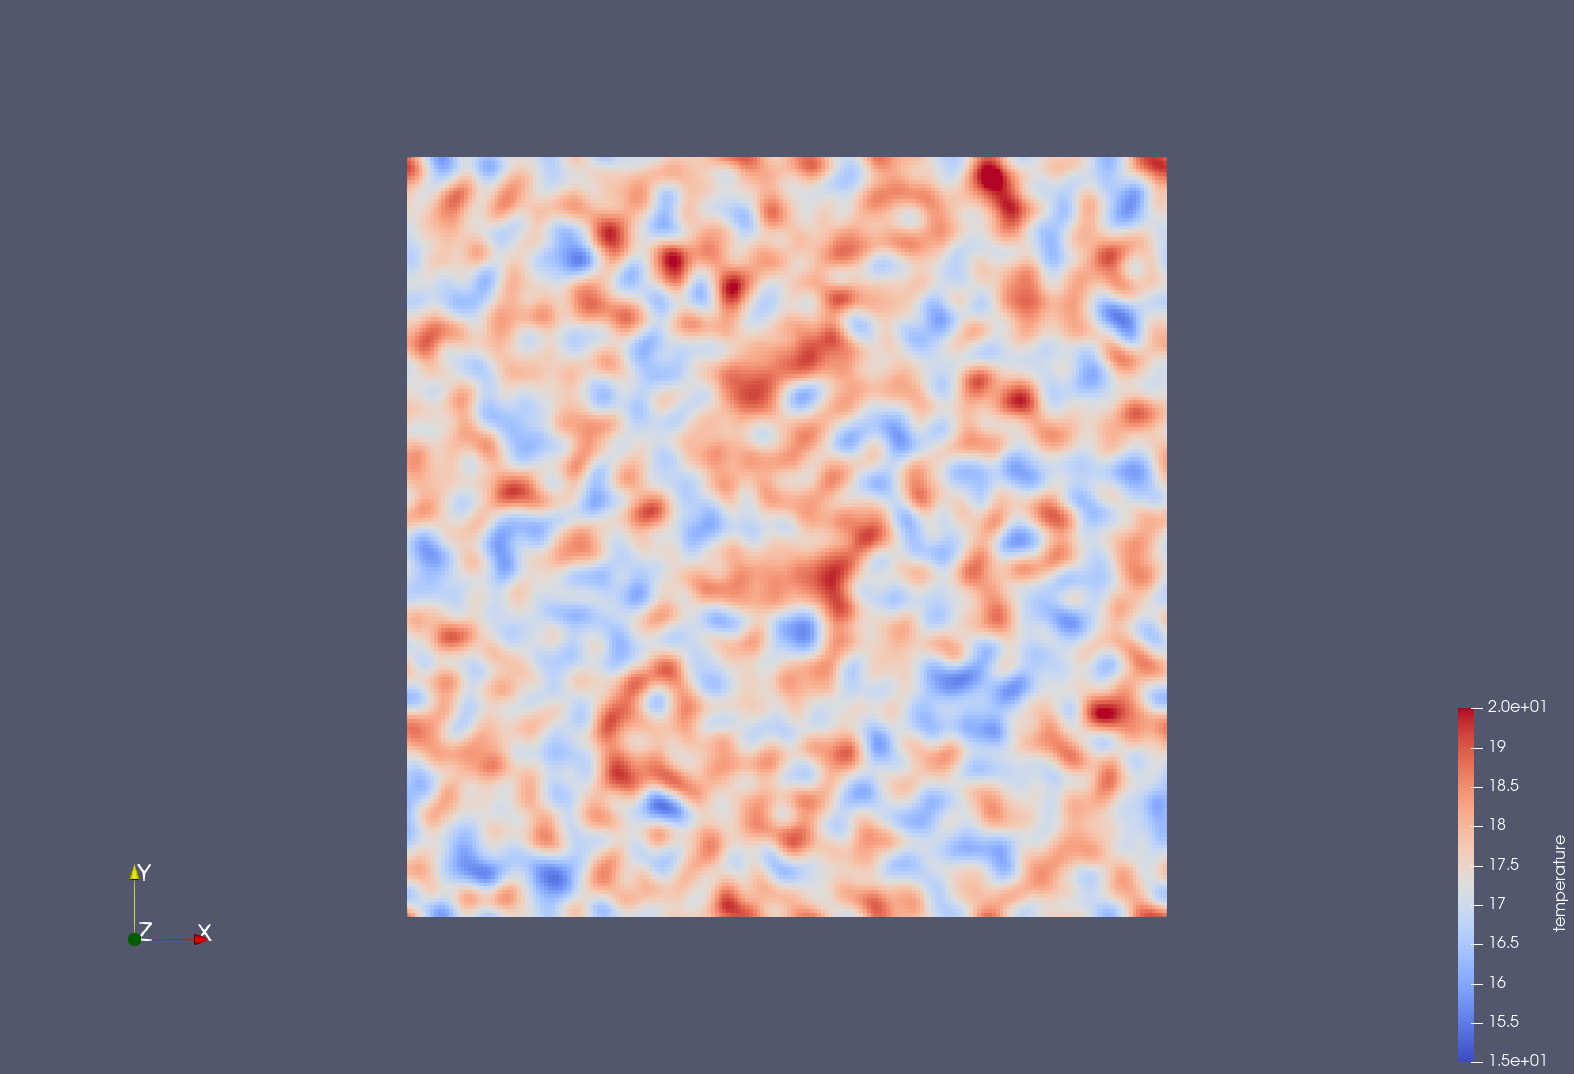
\includegraphics[width=\textwidth]{../images/vtk/bonus/temp/step_50.png}
    \caption{Time step 500}
\end{subfigure}
\hfill
\begin{subfigure}{0.4\textwidth}
    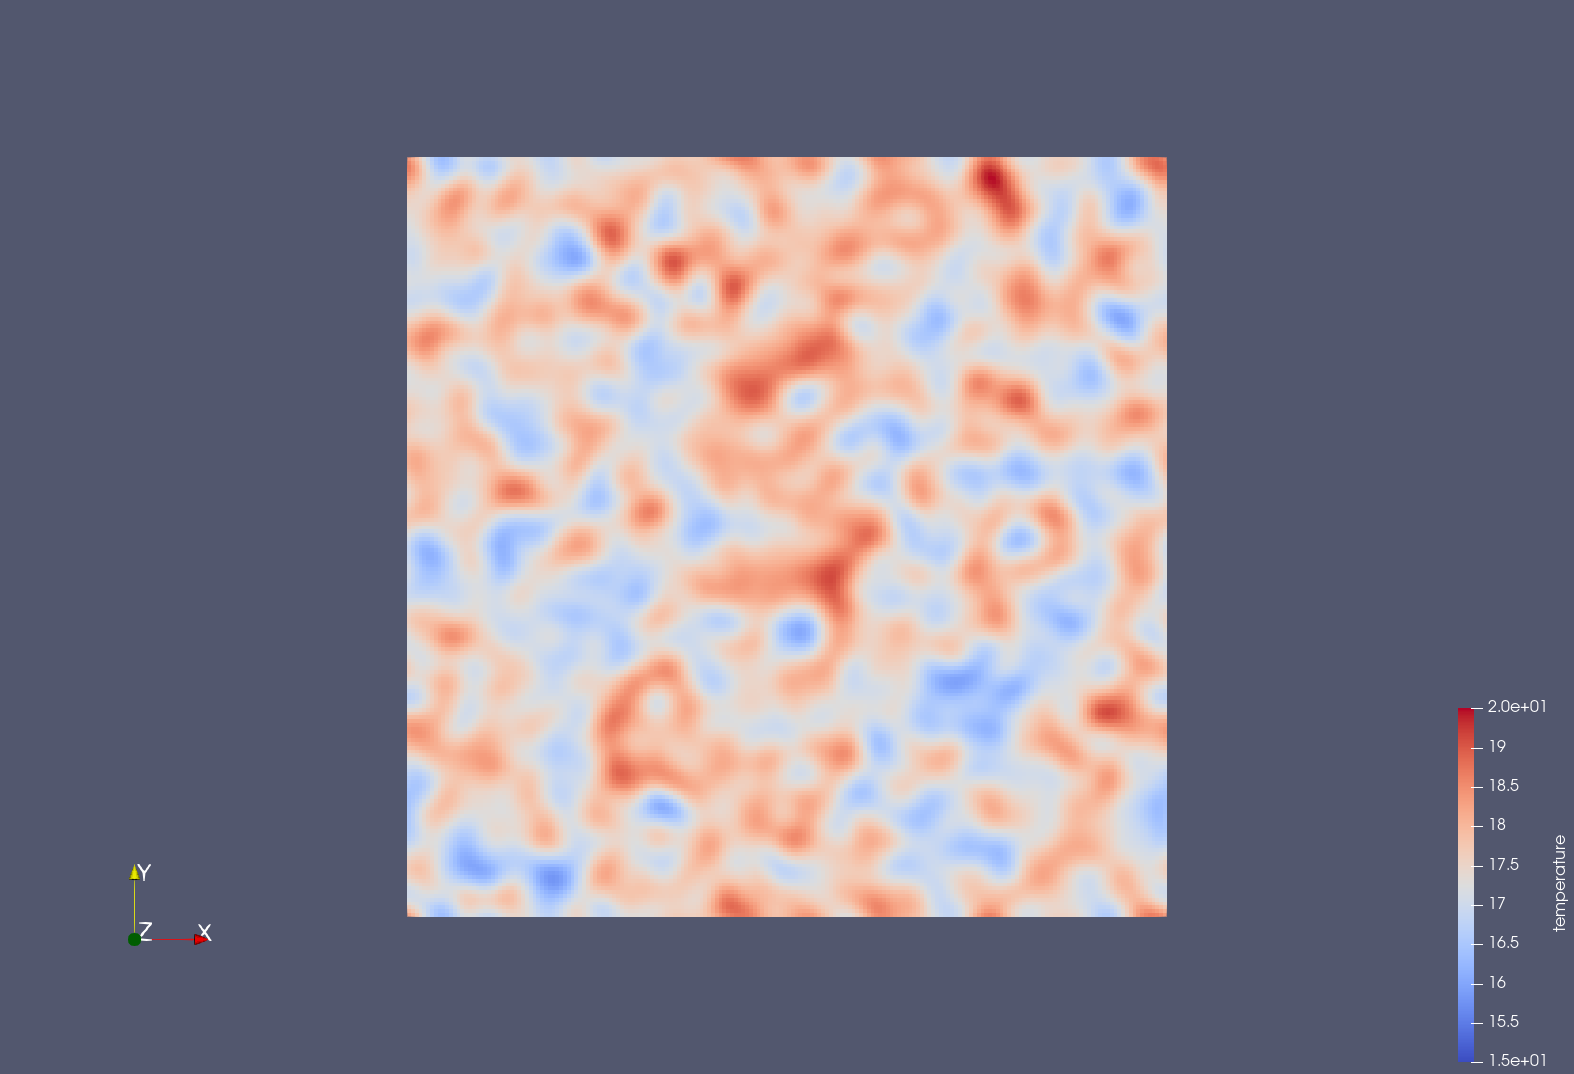
\includegraphics[width=\textwidth]{../images/vtk/bonus/temp/step_75.png}
    \caption{Time step 750}
\end{subfigure}

\begin{subfigure}{0.4\textwidth}
    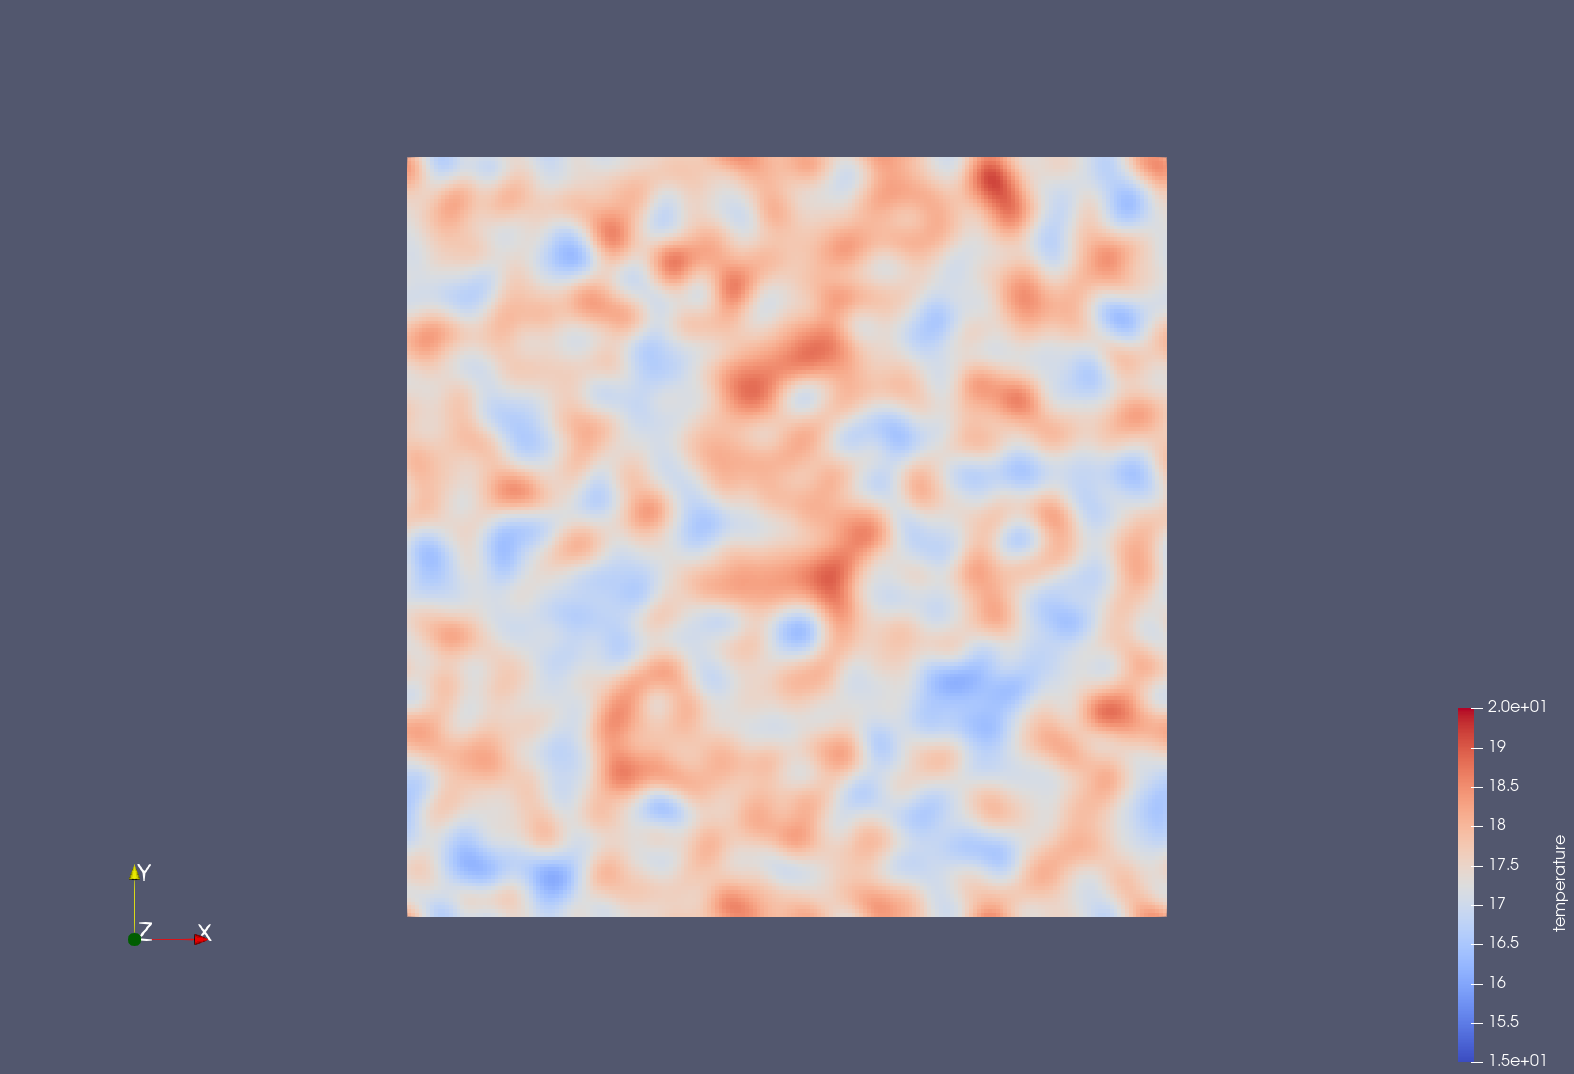
\includegraphics[width=\textwidth]{../images/vtk/bonus/temp/step_100.png}
    \caption{Time step 1000}
\end{subfigure}
        
\caption{Screenshots from Paraview Ocean Temperature Visualization}
\end{figure}

\begin{figure}
\centering
\begin{subfigure}{0.4\textwidth}
    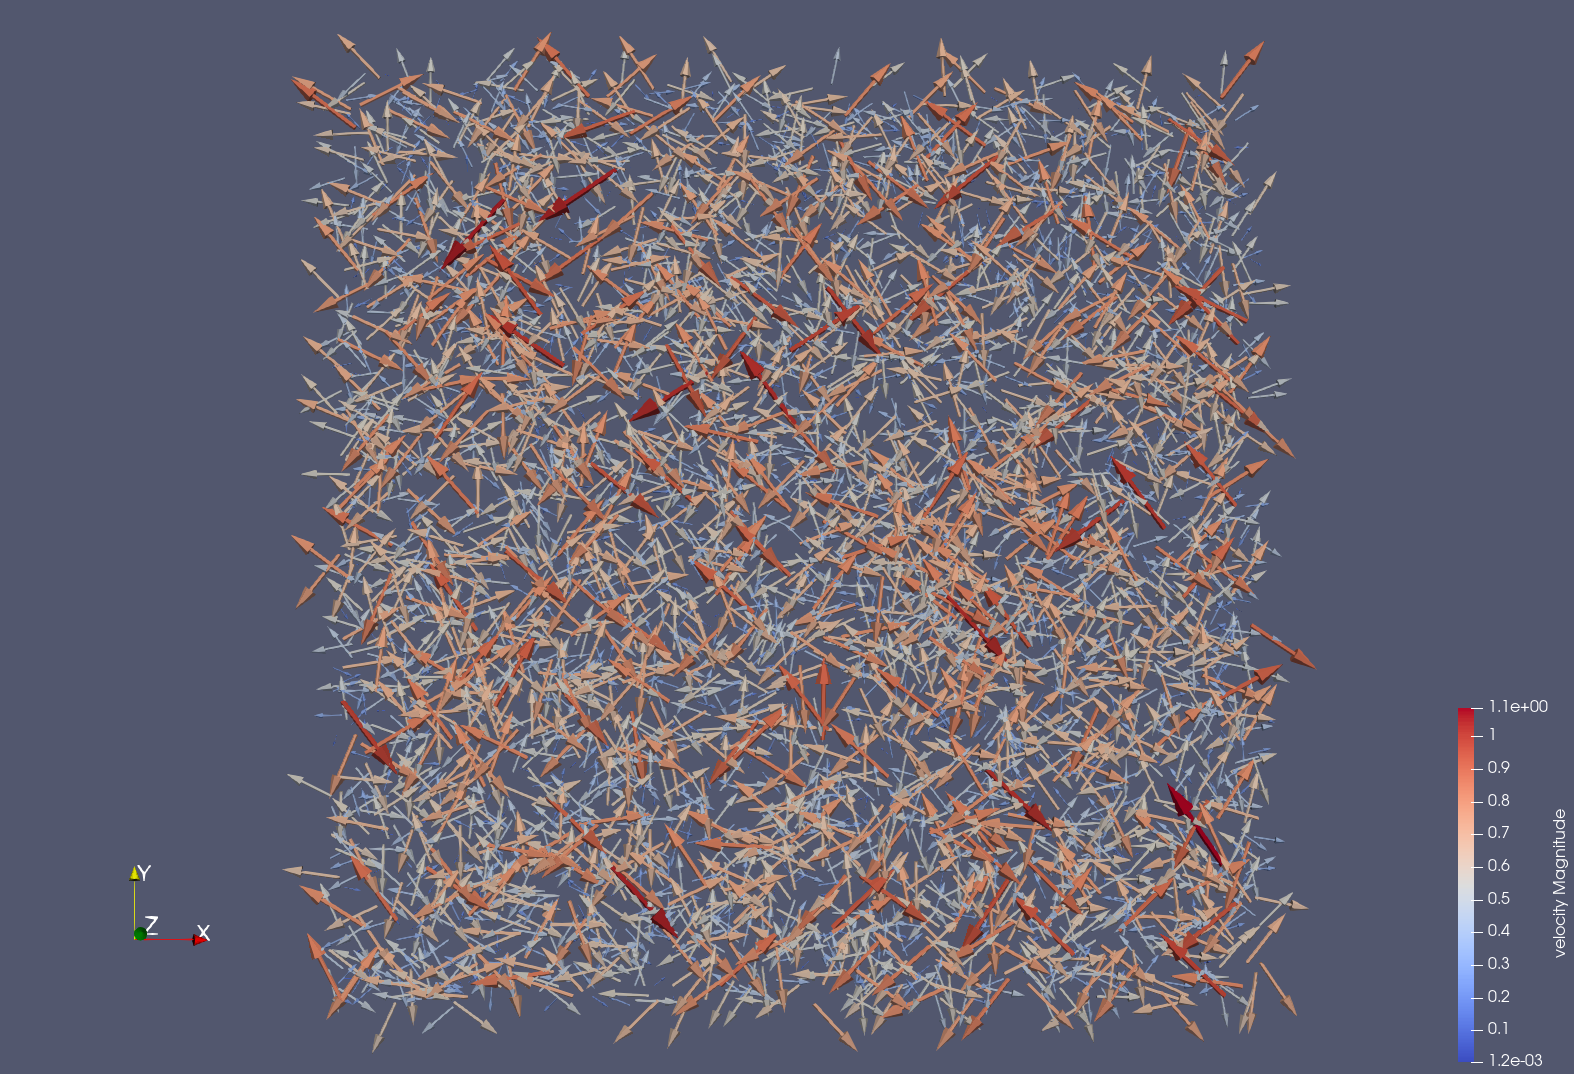
\includegraphics[width=\textwidth]{../images/vtk/bonus/velocity/step_0.png}
    \caption{Time step 0}
\end{subfigure}
\hfill
\begin{subfigure}{0.4\textwidth}
    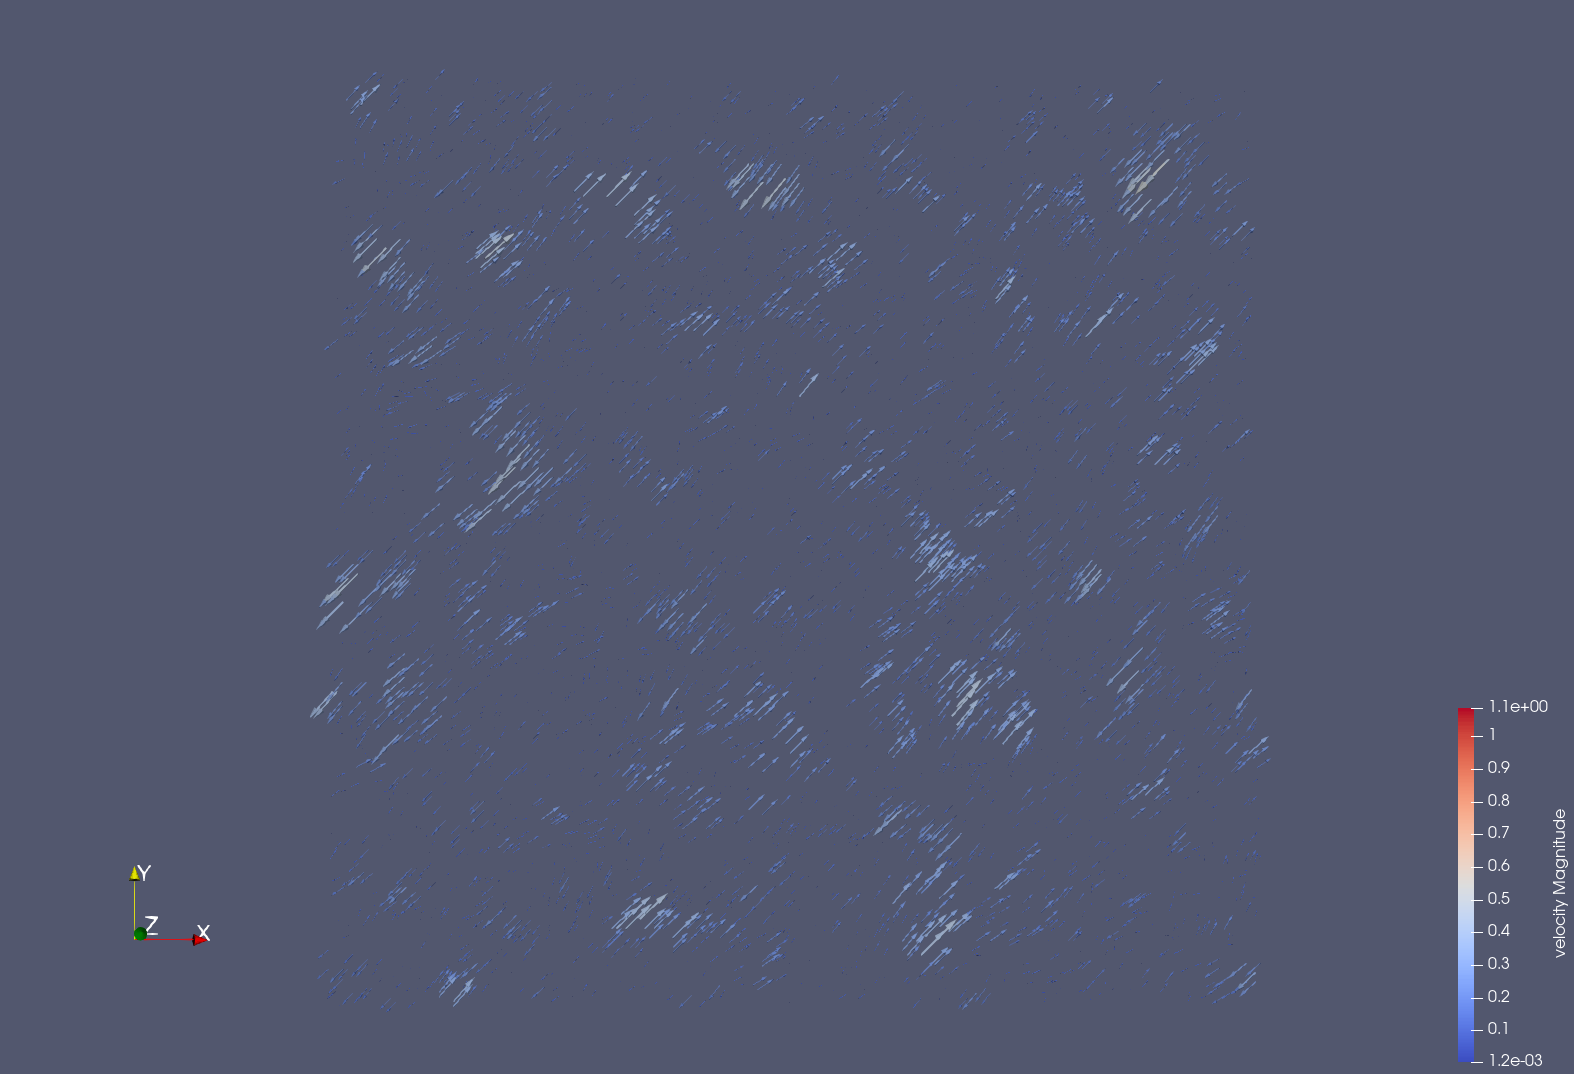
\includegraphics[width=\textwidth]{../images/vtk/bonus/velocity/step_25.png}
    \caption{Time step 250}
\end{subfigure}
\hfill
\begin{subfigure}{0.4\textwidth}
    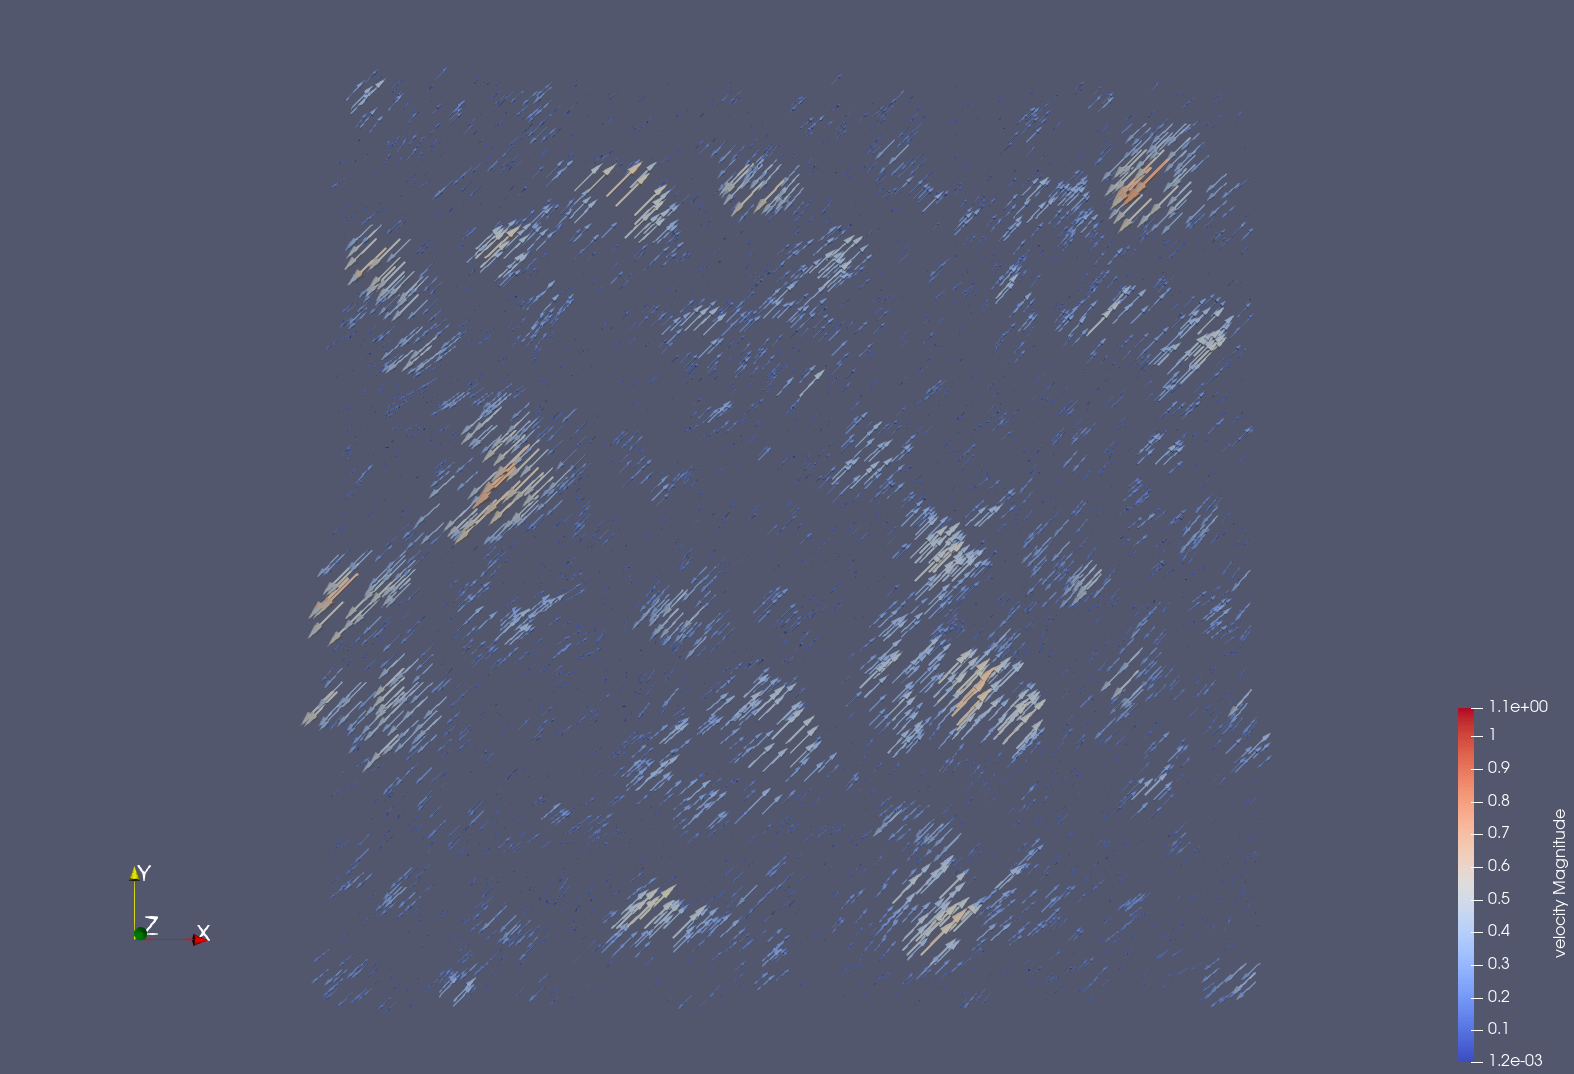
\includegraphics[width=\textwidth]{../images/vtk/bonus/velocity/step_50.png}
    \caption{Time step 500}
\end{subfigure}
\hfill
\begin{subfigure}{0.4\textwidth}
    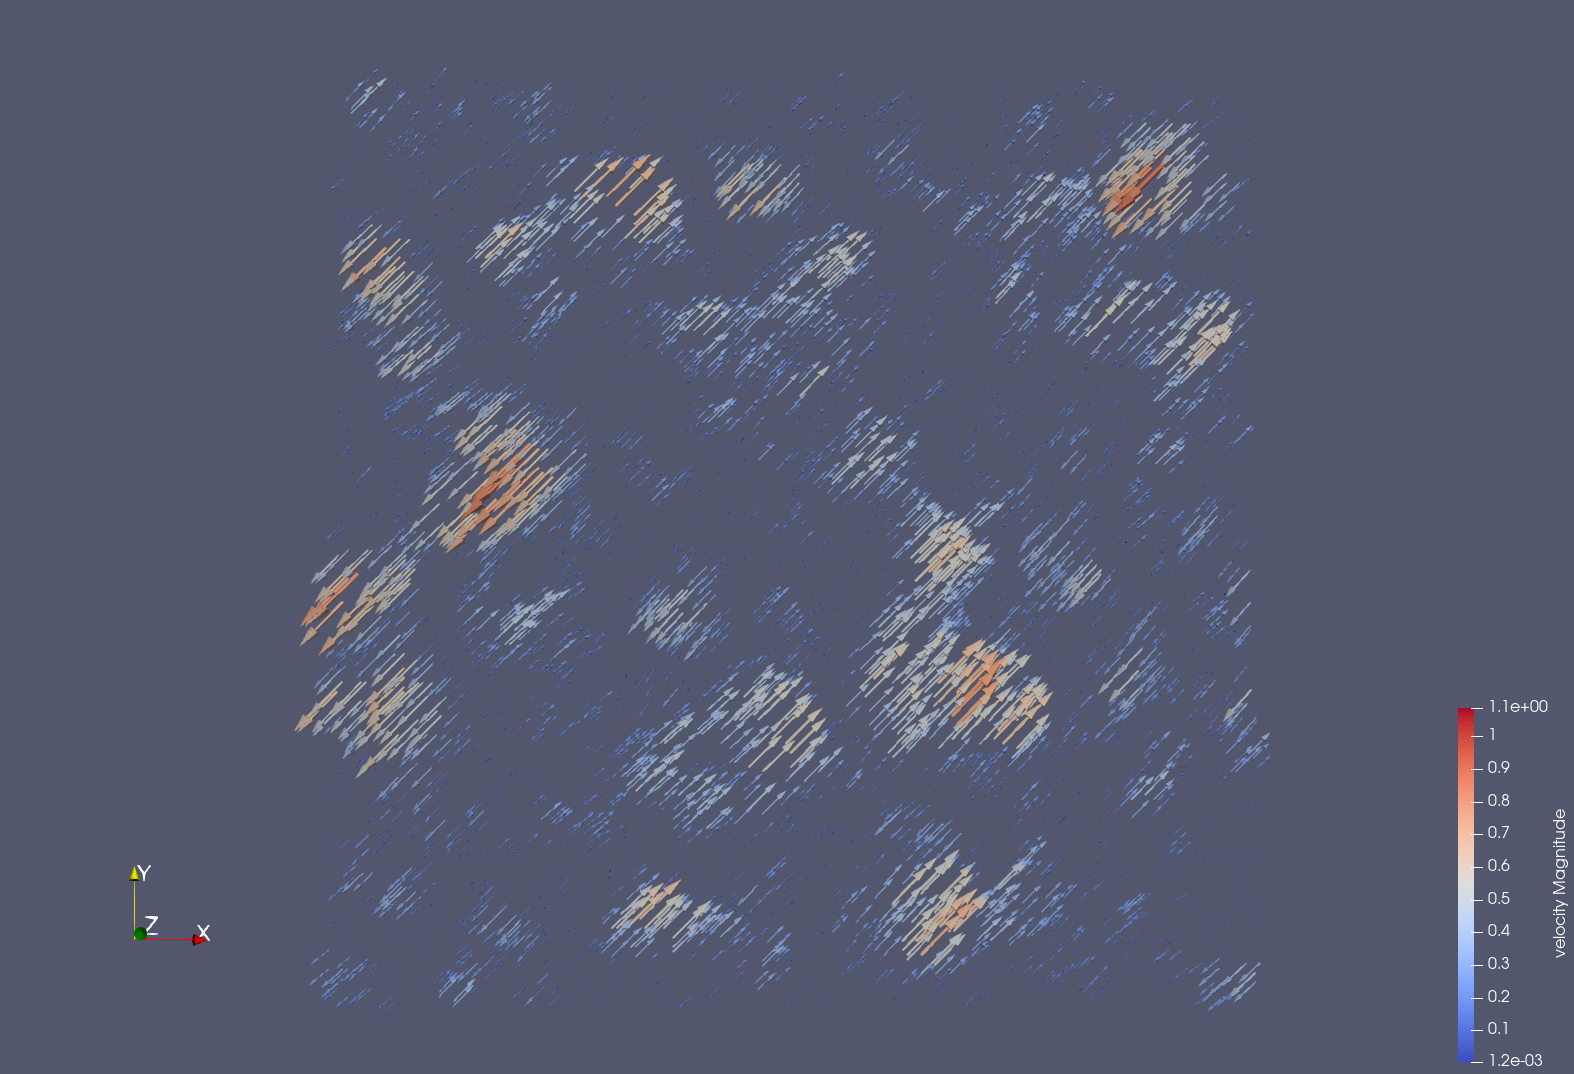
\includegraphics[width=\textwidth]{../images/vtk/bonus/velocity/step_75.png}
    \caption{Time step 750}
\end{subfigure}

\begin{subfigure}{0.4\textwidth}
    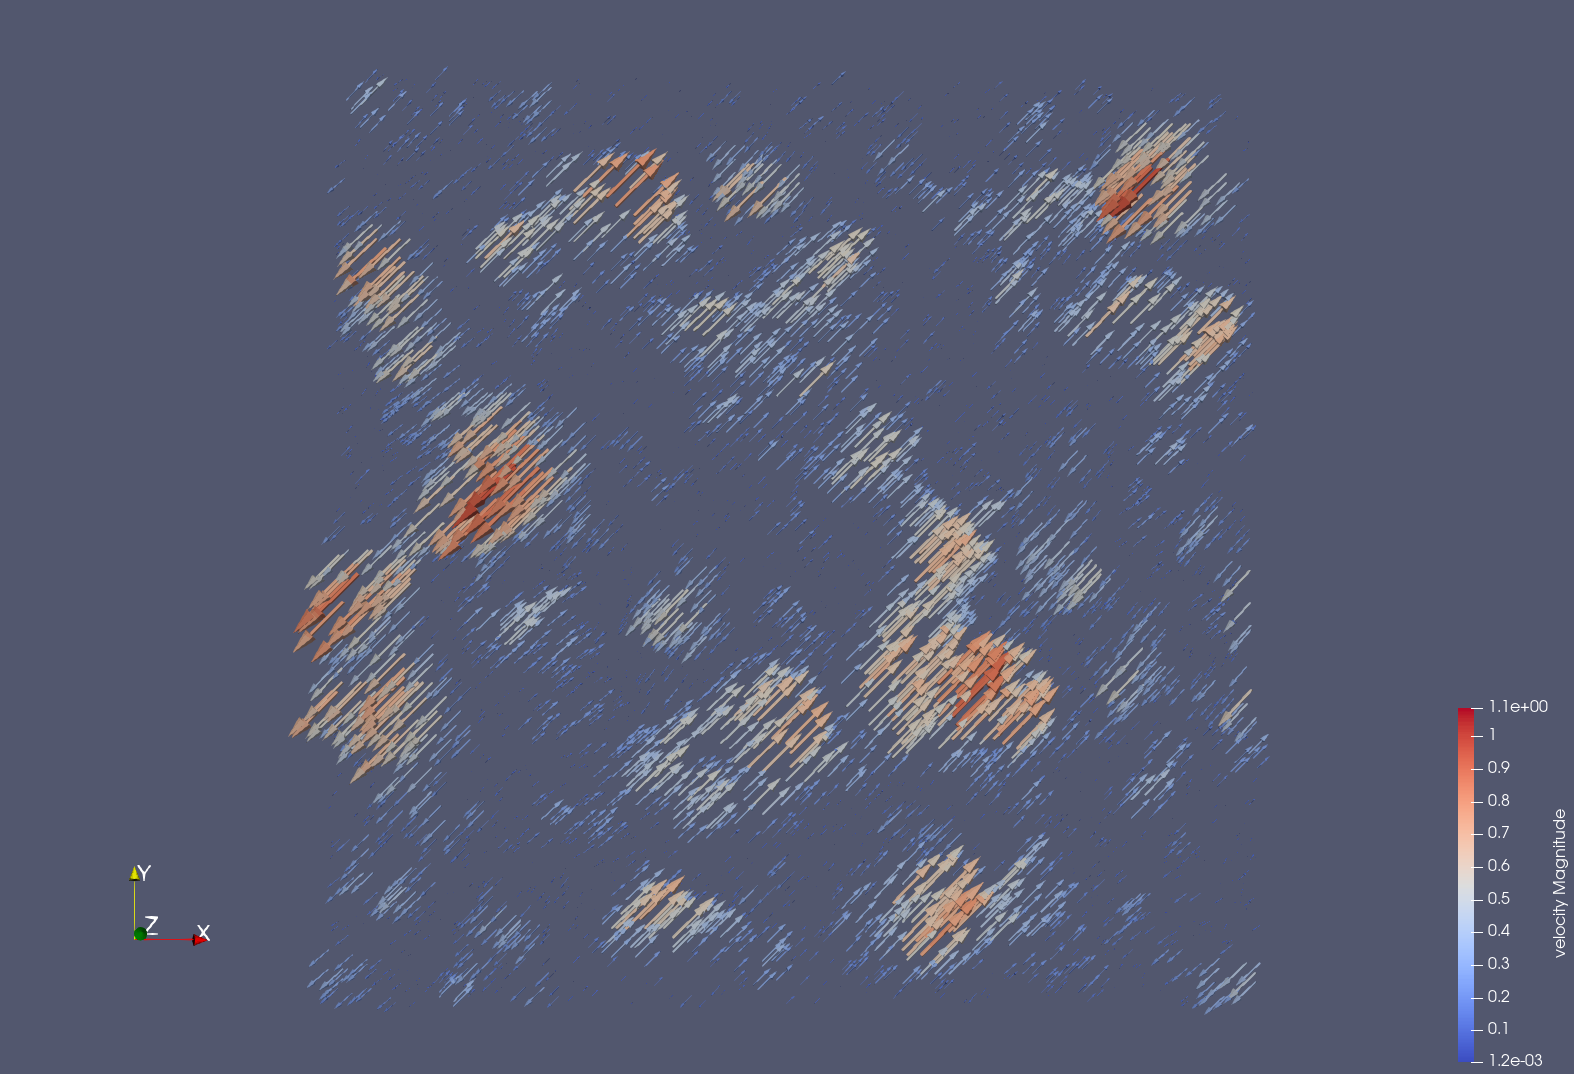
\includegraphics[width=\textwidth]{../images/vtk/bonus/velocity/step_100.png}
    \caption{Time step 1000}
\end{subfigure}
        
\caption{Screenshots from Paraview Ocean Current Velocity Visualization}
\end{figure}


% content end
%###############################################################################

% TODO: bibliograpghy when needed
% \printbibliography

\end{document}
